\section{Preliminary Implementation}\label{Se:experiments}

In this section, we report encouraging results of our prototype implementation.
We have implemented static analysis and the runtime synchronization algorithm, and an experimental evaluation over a set of four real-world subjects. 

%\smartpar{Prototype System}
%\label{Se:system}
We have created a Java implementation of our static analysis for composed {\sf Map} operations, as described  in Section \ref{se:instance}. Given $n$ types of transactions, our implementation builds a serialized CFG as described in Section \ref{Se:concabs}, and then it computes a fixpoint over it relying on the abstract semantics formalized in Section \ref{sect:abstractsemantics}. We support all the operations listed in Section \ref{sect:language}. Running times are negligible compared to the rest the process, and the analysis converges always in less than a second. Therefore, we do not report the running times of the static analysis.

As explained earlier, the interface with the runtime system is a relational corrective specification mapping prestates to sets of poststates that are obtainable via serializable execution of the transactions from the prestate. As a partial example, 
%\begin{center}
$[ {\sf k} \mapsto \bot , {\sf v} \mapsto v ] \leadsto \{ [ {\sf k} \mapsto v , {\sf v} \mapsto v ] \}$
%\end{center}
denotes that if we started from a prestate where ${\sf k}$ was not in the map and the value passed to the function was $v$, then in the poststate the key ${\sf k}$ is made to point to the value $v$ pointed-to by the second argument ${\sf v}$ in the prestate.
%
The runtime system $S$ is parameterized by the specification, which it loads at the beginning of the concurrent run. 

As discussed in Section \ref{sec:dynamicwarping}, in our current prototype all transactions are assumed to start simultaneously. This is useful, for example, in loop parallelization. Each concrete transaction is mapped to its abstract counterpart, as explained in Section \ref{Se:concabs}. The mapping process also binds the concrete arguments of the transaction (i.e., the concrete object references) to their symbolic counterparts (e.g., the {\sf k} and {\sf v} symbols above). 

During execution, the runtime system monitors commit events. In our current prototype, we limit transactions to a single commit point before completion. Corrective synchronization occurs only on failed commits (as discussed in Section \ref{Se:guarantees}), in which case the transaction's shared log, local state and return value (if it exists) are all (potentially) modified according to the corrective specification. 

\OmerAdded{Analogously to the pruning technique used to map between states and their corrective counterparts, the decision whether a commit has failed is based on incremental pruning of the good global states $G$ according to the final states of committed transactions. If the final state of a transaction is not consistent with state $g \in G$, then $g$ is pruned out. If $G$ at any point becomes empty, then the system has reached a bad state.}

\smartpar{Methodology and Experimental Setup}
%
We conducted our experiments on server with two Intel(R) Xeon(R) CPU E5-2690 0 @ 2.90GHz (16 cores) CPUs with 132GB of RAM. The server runs version
6.6 of the CentOS Linux distribution, and has the Sun 64-Bit 1.8 Java virtual machine (JVM) installed.

In our experiments, we varied two aspects of parallel execution: \emph{workload size}, measured as the number of transactions executed by a given thread for a fixed number $n$ of threads, and \emph{concurrency level}, setting the number of threads for a fixed workload size. For the former, we fixed $n=8$ and varied the number of transactions, where each transaction executes a single client method. For the latter, we experimented with 2 to 32 threads with workload size fixed at 10.
%\begin{itemize}
	%\item
%	\emph{Workload size:} For a fixed number $n$ of threads, where $n=8$,  the workload size is varied. The workload is measured as the number of transactions executed by a given thread, where a single transaction consists of the invocation of a particular method. All inputs share the same key(s).
%	\item \underline{Concurrency level:} For a fixed workload size, set at 10%\pengtodo{please confirm}
%	, the number of threads is varied along the range of 2 to 32 threads.  
%\end{itemize}
For statistical soundness, we report the average performance results across 10 independent repetitions of each experiment.

We compare our technique against two competing solutions: (i) a pessimistic concrete-level variant of STM, as available via version 1.3 of the Deuce STM (the latest version)\footnote{
		\url{https://github.com/DeuceSTM/DeuceSTM}
	}, and (ii)  a lock-based synchronization algorithm boosted with {\sf Map} semantics \cite{ppopp/HerlihyK08}, such that the locks are of the same grain as their corresponding abstract locks in boosted STM.

\smartpar{Subjects}
%
Our benchmark suite consists of four subjects, all of which are taken from popular open-source code bases and have been used in past studies on concurrency \cite{oopsla/ShachamBASVY11,issta/ShachamYGABSV14}.
%\begin{itemize}
	%\item 
	Apache Tomcat is web-app container in wide deployment. Within it, we consider {\sf ApplicationContext}, which is a concrete representation of a web application's execution environment.
	dyuproject is a framework for development of Java web applications. We experiment with {\sf StandardConvertorCache}, which handles conversion of objects to/from JSON format.
	Flexive is a next-generation content repository for development of web apps, in particular in an enterprise setting. We have included {\sf FxValueRendererFactory} from it, which is responsible to render transparently certain objects in a language.
	Finally, Gridkit is a library containing utilities related to in-memory data grids. In it, {\sf ReflectionPofSerializer} is a concurrent data structure that supports generic POF serialization via reflection.
%\end{itemize}

We have extracted two concurrent methods out of each benchmark. These were selected based on past studies that report on concurrency bugs in, and interference between, the selected methods \cite{oopsla/ShachamBASVY11}. 
%
As an illustration, in Figure \ref{Fi:gridkitPair} we present the method pair from Gridkit. In both of these methods, the intended atomic ``put-if-absent'' behavior (available as the {\sf putIfAbsent} API) is misimplemented due to the separation between the {\sf get} and {\sf put} calls. (We omit other method pairs for lack of space.)

\begin{figure}[tb]
%	\begin{lstlisting}
%protected Object internalDeserialize(PofReader in) 
%   throws IOException {
% Class type = in.getPofContext().getClass(in.getUserTypeId());
% ObjectFormat format = formats.get(type);
% if (format == null) {
%  try {
%   format = new ObjectFormat(type);
%  } catch (Exception e) {
%   throw new IOException(... + type.getName(), e); }
%  formats.put(type, format); }
%  Object result = resolve(format.deserialize(in));
%  return result; }
%	\end{lstlisting}
%
%	\begin{lstlisting}
%protected void internalSerialize(PofWriter out,Object origVal) 
%   throws IOException {
% Object value = replace(origVal);
% Class type = value.getClass();
% ObjectFormat format = formats.get(type);
% if (format == null) {
%  try {
%   format = new ObjectFormat(type);
%  } catch (Exception e) {
%   throw new IOException(... + type.getName(), e); }
%  formats.put(type, format); }
% format.serialize(out, value); }
%	\end{lstlisting}
\begin{lstlisting}
Object internalDeserialize(PofReader in) {
  Class t = in.getPofContext().getClass(in.getUserTypeId());
  ObjectFormat f = formats.get(t);
  if (f == null) { f = new ObjectFormat(t); formats.put(t, f); }
  return resolve(f.deserialize(in)); }

void internalSerialize(PofWriter out, Object o) {
  Object v = replace(o); Class t = v.getClass();
  ObjectFormat f = formats.get(t);
  if (f == null) { format = new ObjectFormat(t); formats.put(t, f); }
  format.serialize(out, v); }
\end{lstlisting}
	\caption{\label{Fi:gridkitPair}Concurrent methods from the Gridkit benchmark}
\end{figure}


\begin{figure*}
	\begin{minipage}{0.50 \textwidth}
		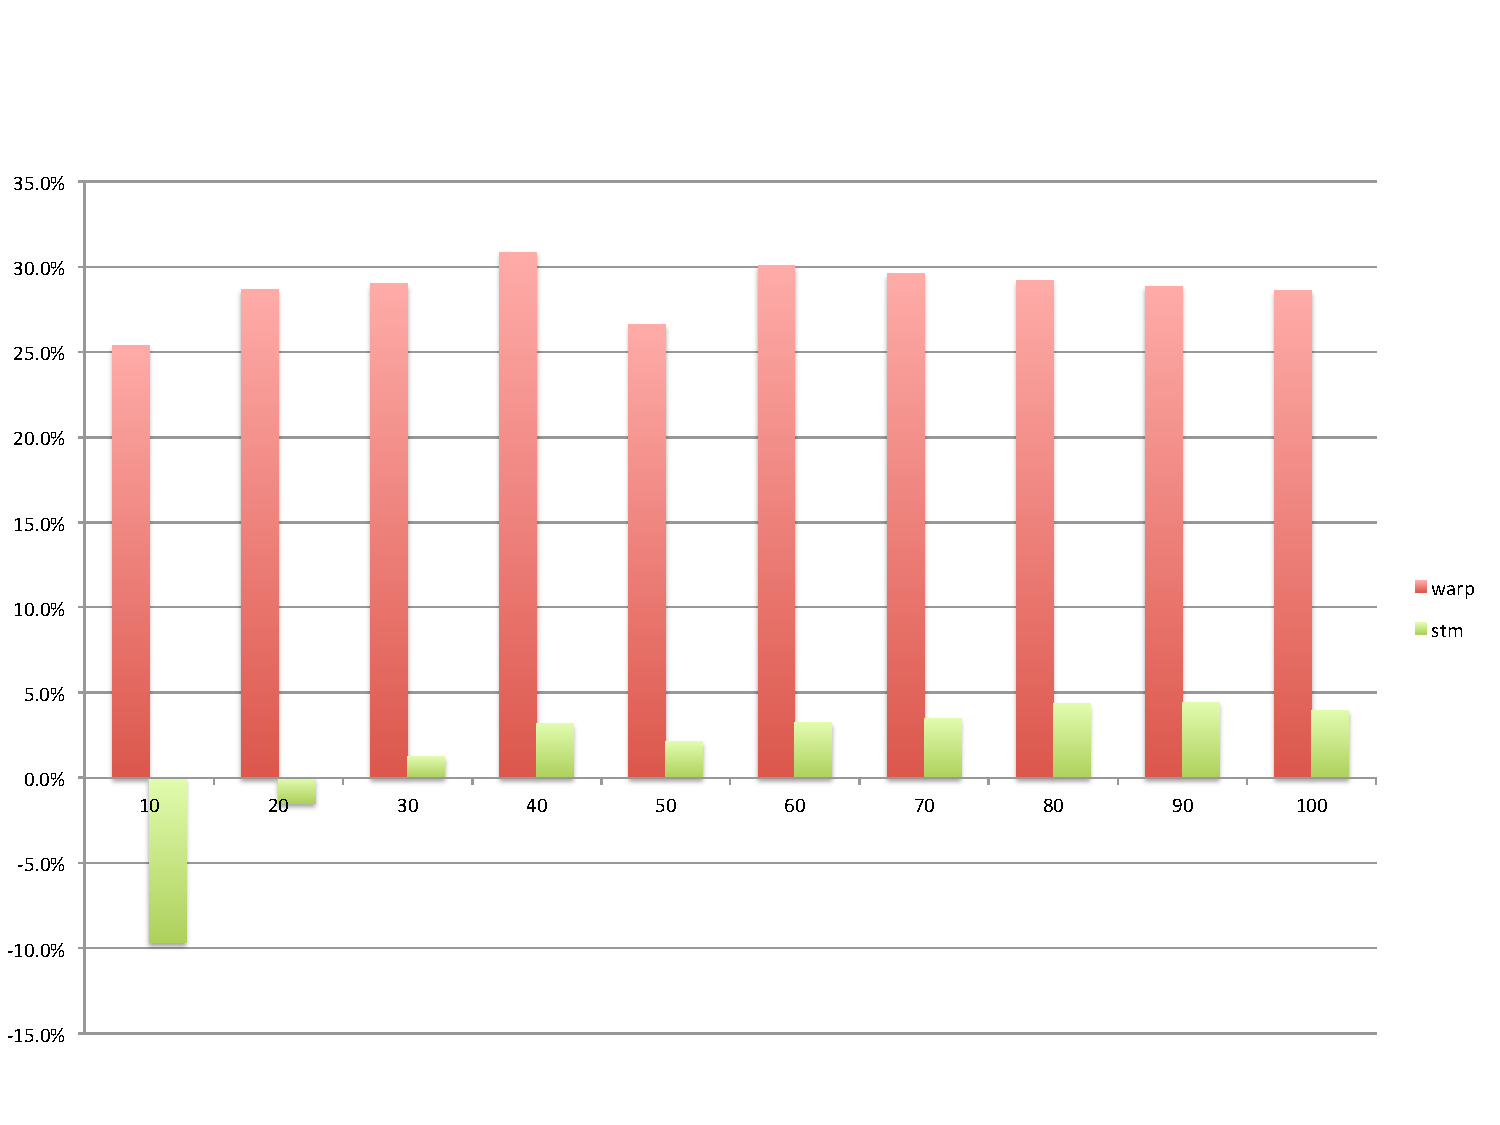
\includegraphics[width=0.5 \textwidth]{../../eval/32threads/case1it.pdf}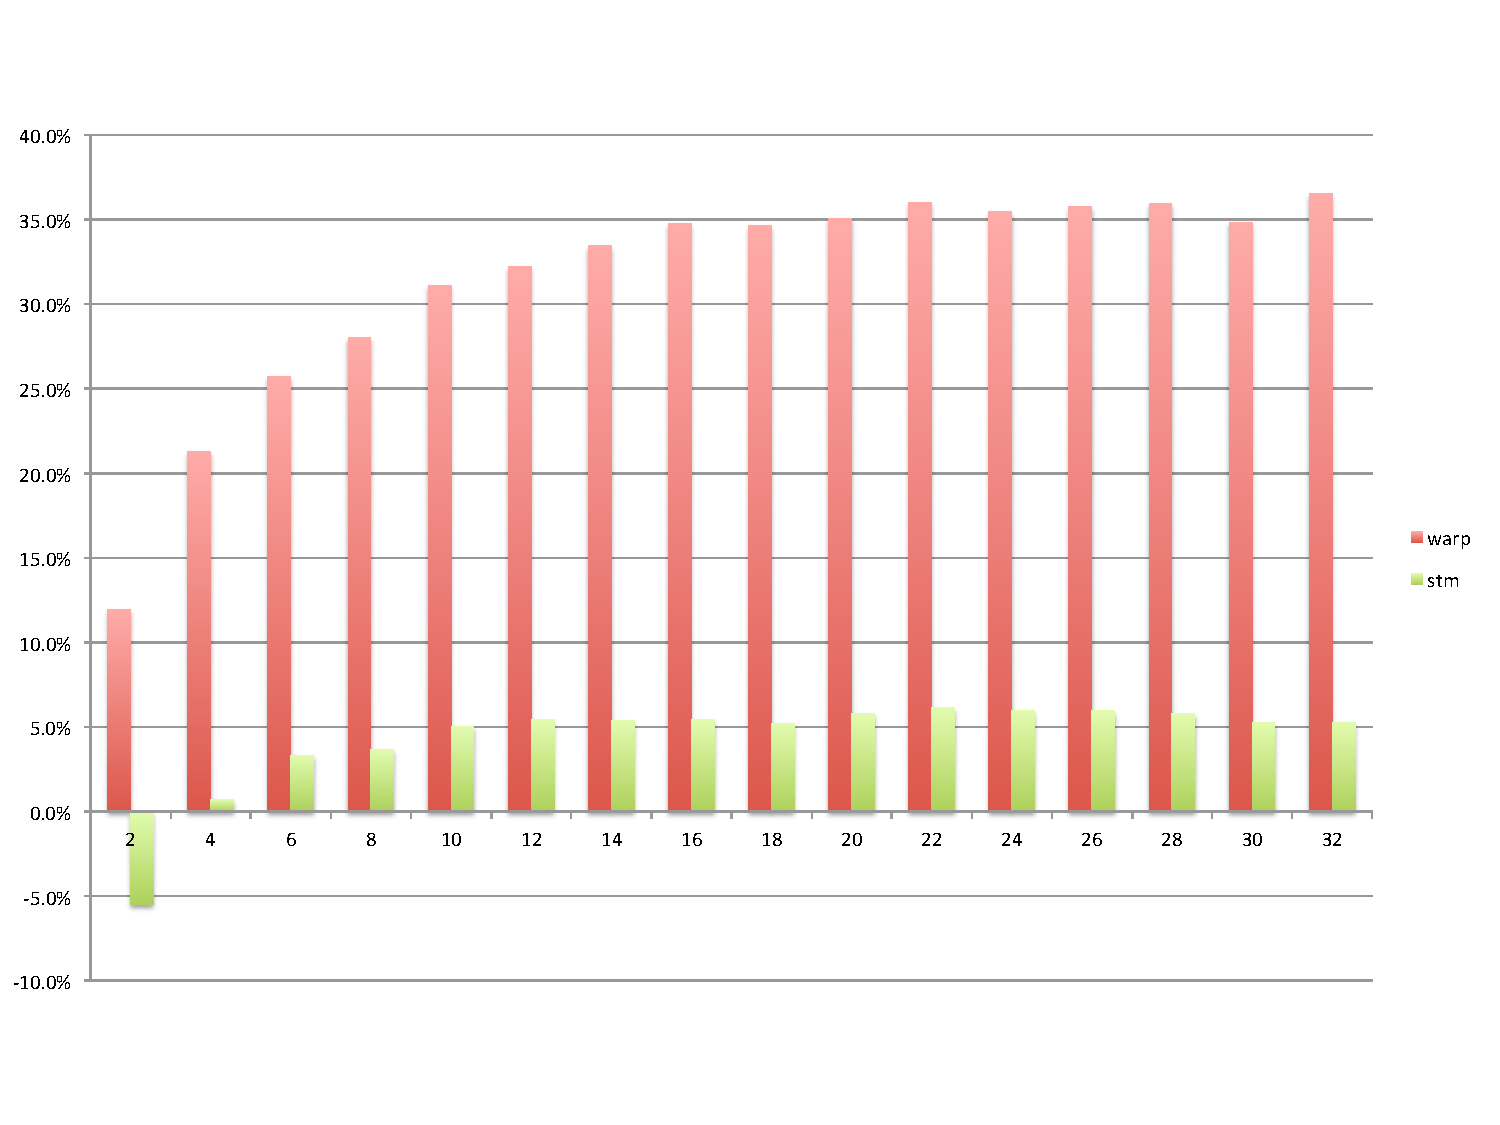
\includegraphics[width=0.5 \textwidth]{../../eval/32threads/case1th.pdf}
		\caption{\label{Fi:case1th}Apache Tomcat {\sf ApplicationContext} (l: workload; r: conc)\vspace{10pt}}
	\end{minipage}
	\hfill
	\begin{minipage}{0.5 \textwidth}
		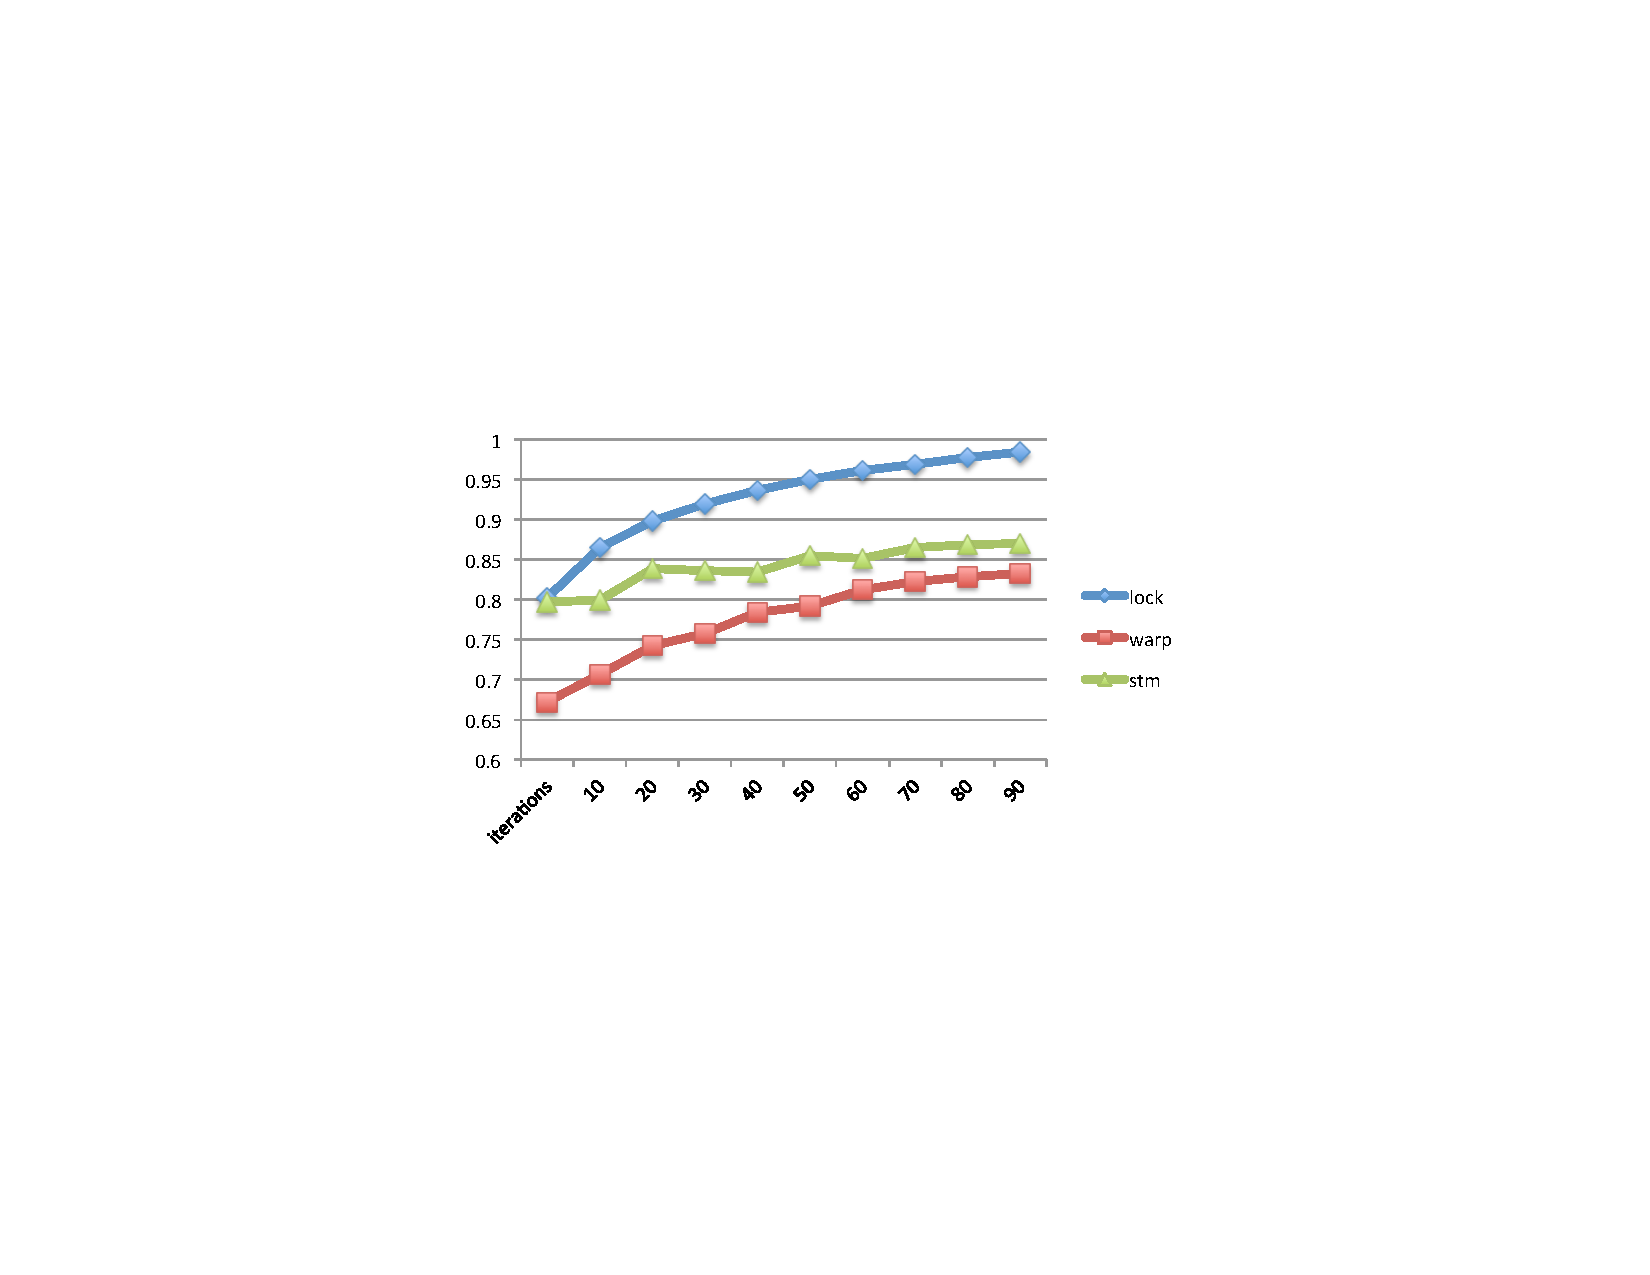
\includegraphics[width=0.5 \textwidth]{../../eval/32threads/case2it.pdf}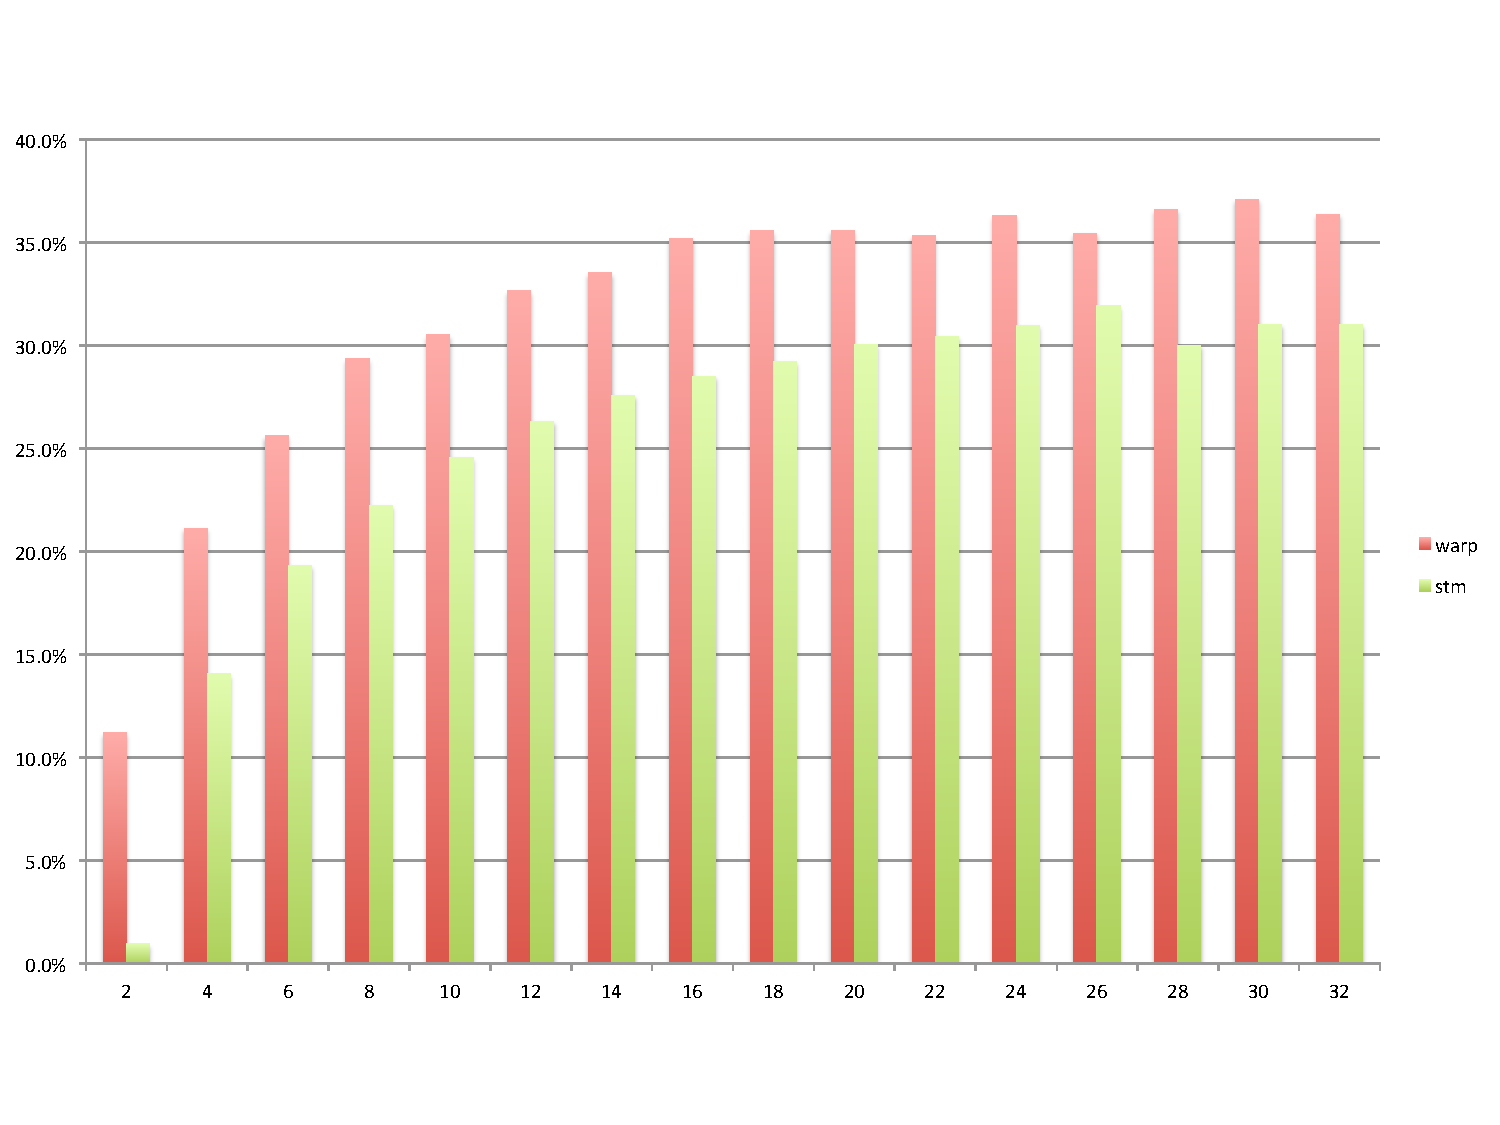
\includegraphics[width=0.5 \textwidth]{../../eval/32threads/case2th.pdf}
		\caption{\label{Fi:case2th}dyuproject {\sf StandardConvertorCache} 
			(l: workload; r: conc)\vspace{10pt}}
	\end{minipage}
	\begin{minipage}{0.5 \textwidth}
		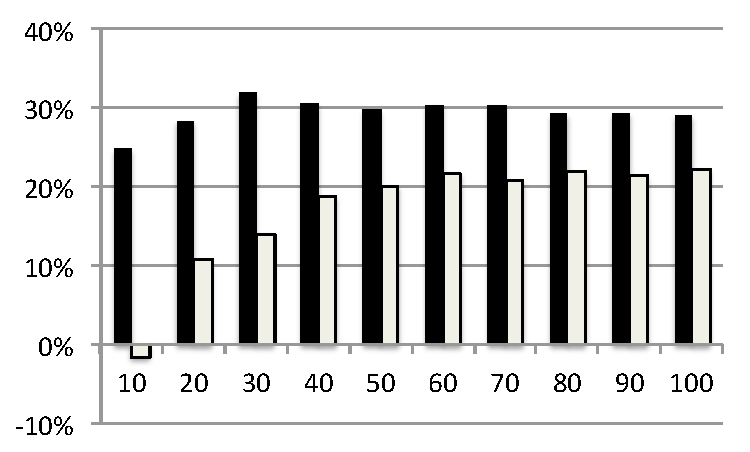
\includegraphics[width=0.5 \textwidth]{../../eval/32threads/case3it.pdf}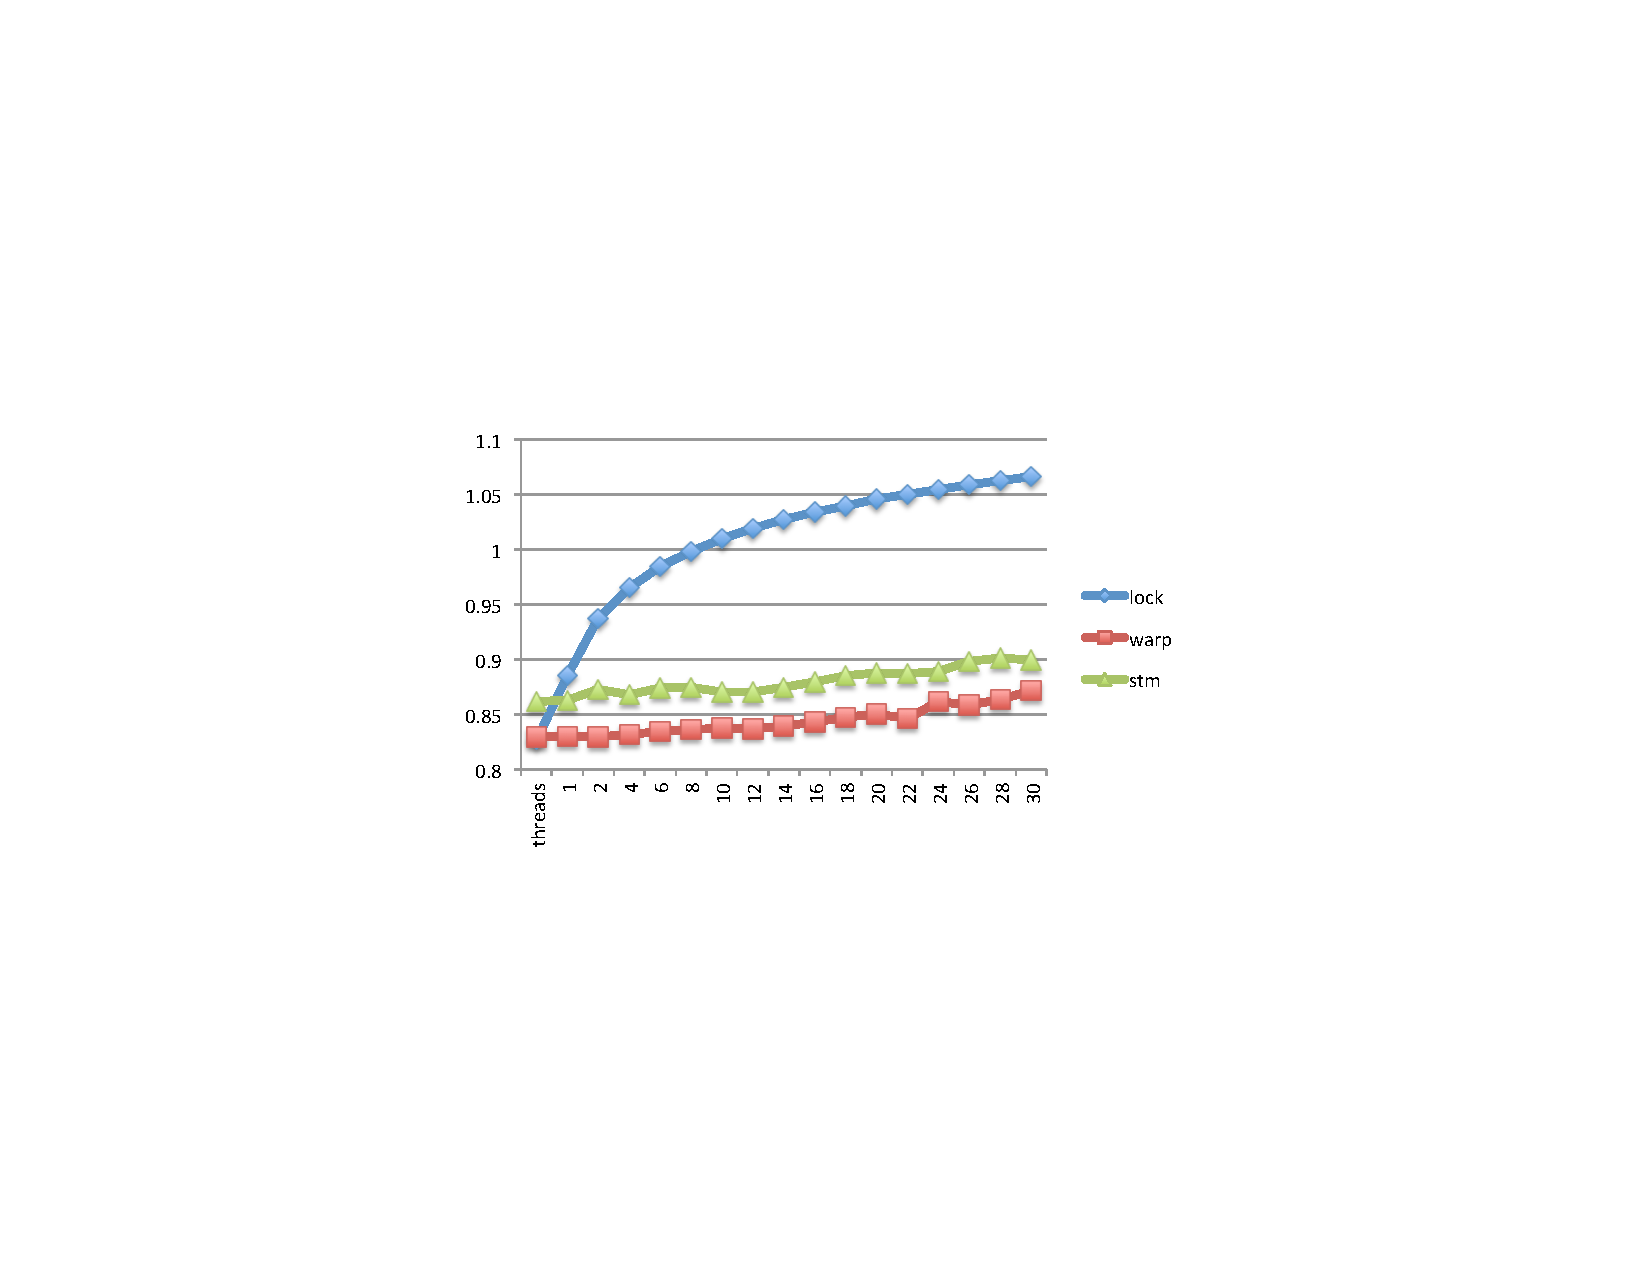
\includegraphics[width=0.5 \textwidth]{../../eval/32threads/case3th.pdf}
		\caption{\label{Fi:case3th}Flexive {\sf FxValueRendererFactory} 
			(l: workload; r: conc)}
	\end{minipage}
	\hfill
	\begin{minipage}{0.5 \textwidth}
		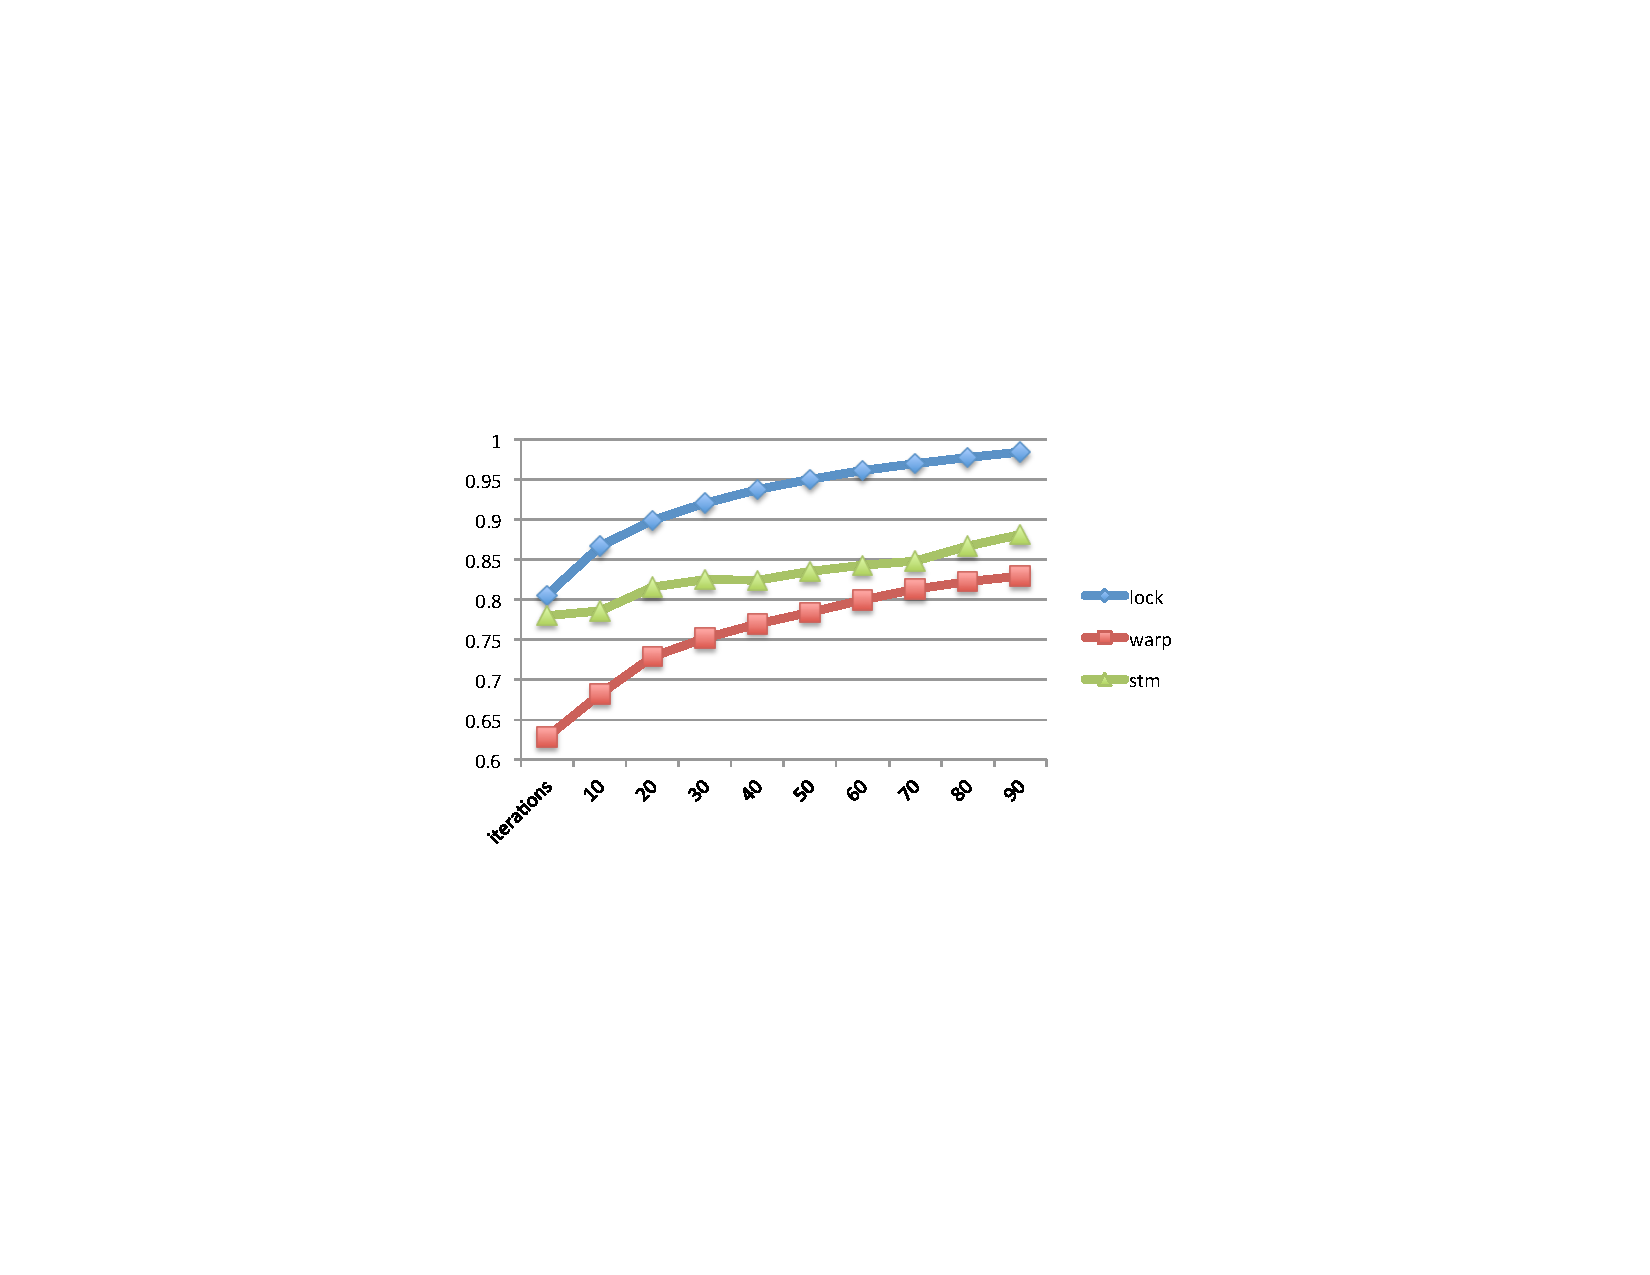
\includegraphics[width=0.5 \textwidth]{../../eval/32threads/case4it.pdf}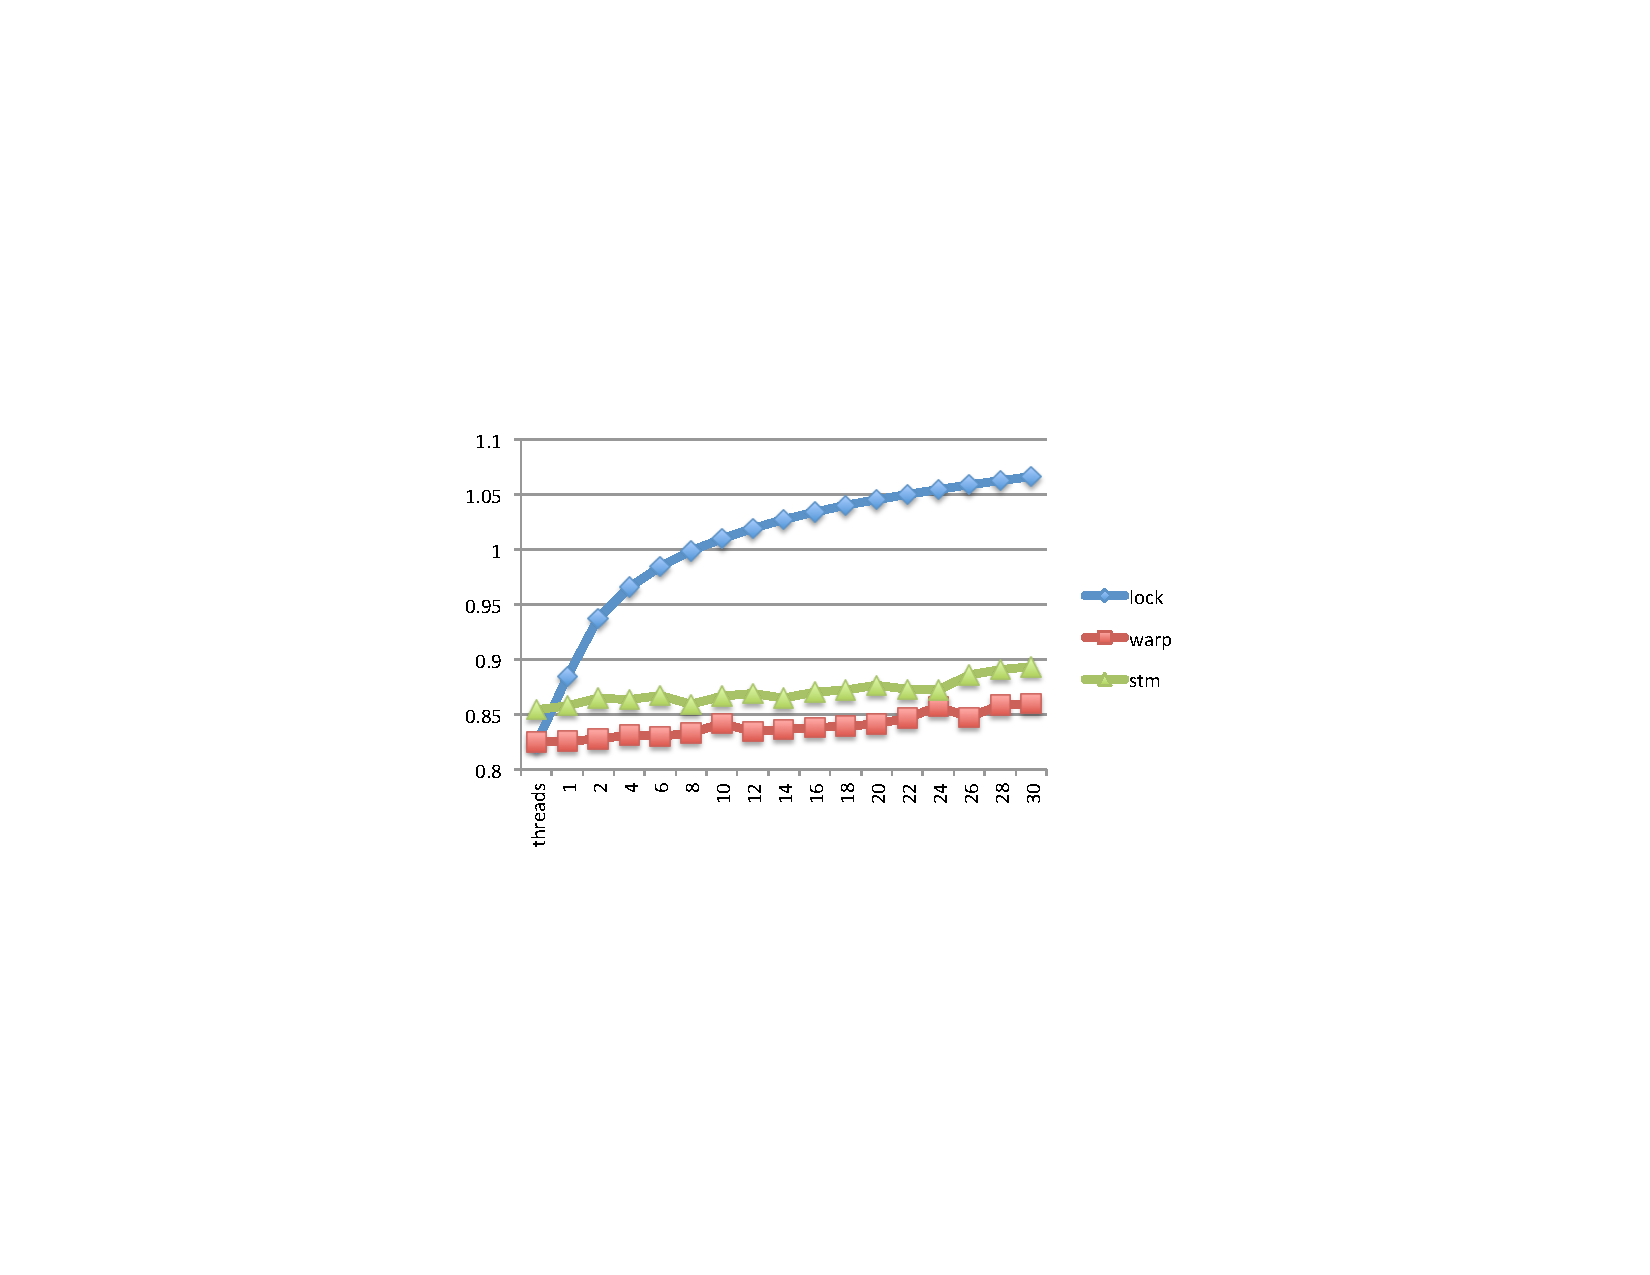
\includegraphics[width=0.5 \textwidth]{../../eval/32threads/case4th.pdf}
		\caption{\label{Fi:case4th}Gridkit {\sf ReflectionPofSerializer}
			(l: workload; r: conc)}
	\end{minipage}
%	
%	\begin{minipage}{0.3 \textwidth}
%		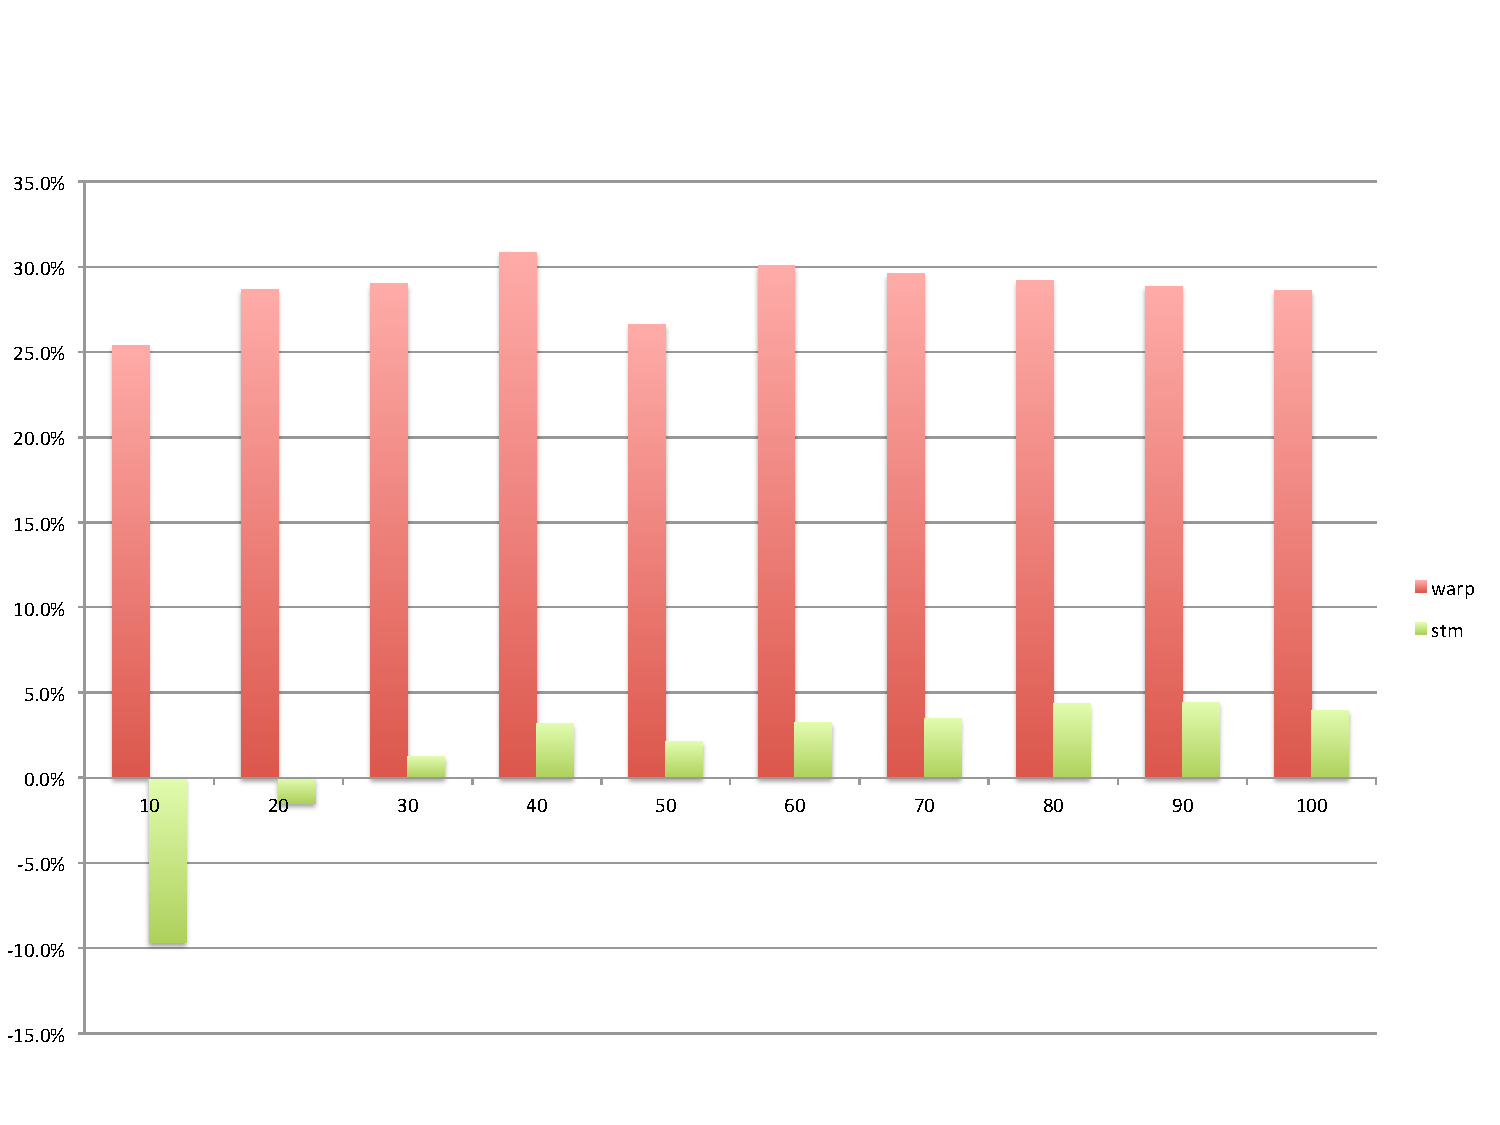
\includegraphics[width=\textwidth]{../../eval/32threads/case1it.pdf}
%		\caption{\label{Fi:case1th}Apache Tomcat {\sf ApplicationContext}: workload}
%	\end{minipage}
%	\hspace{0.05 \textwidth}
%	\begin{minipage}{0.3 \textwidth}
%		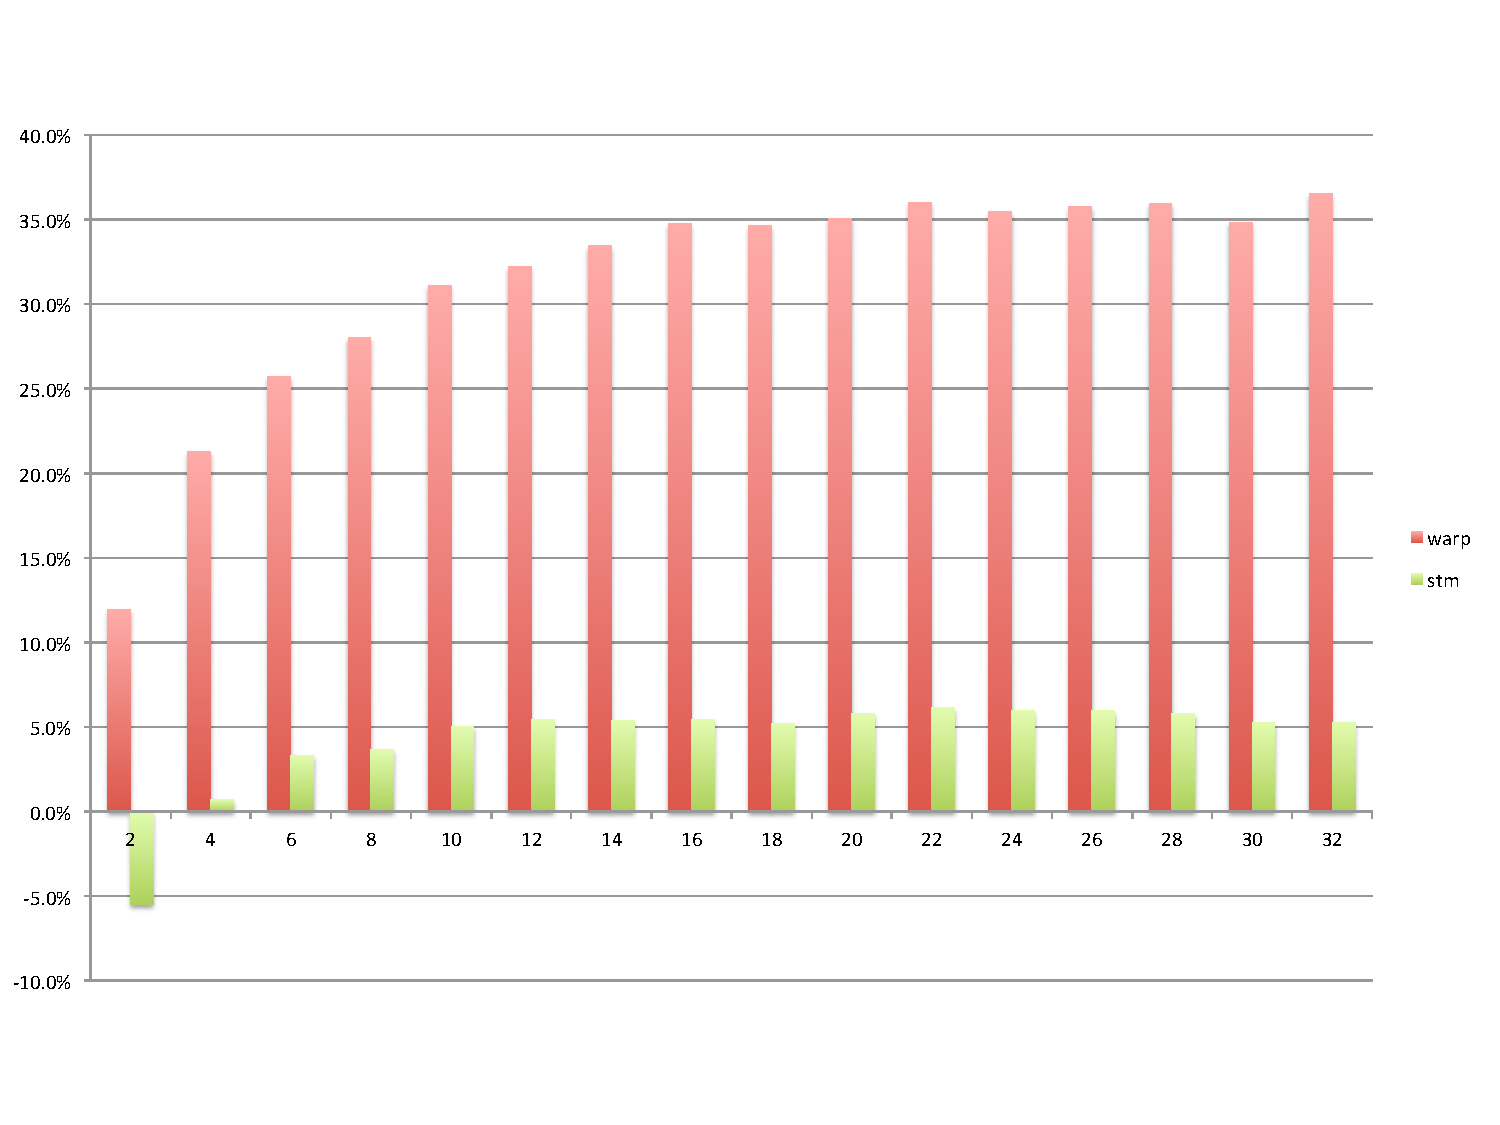
\includegraphics[width=\textwidth]{../../eval/32threads/case1th.pdf}
%		\caption{\label{Fi:case1th}Apache Tomcat {\sf ApplicationContext}: concurrency}
%	\end{minipage}
%	\hspace{0.05 \textwidth}
%	\begin{minipage}{0.3 \textwidth}
%		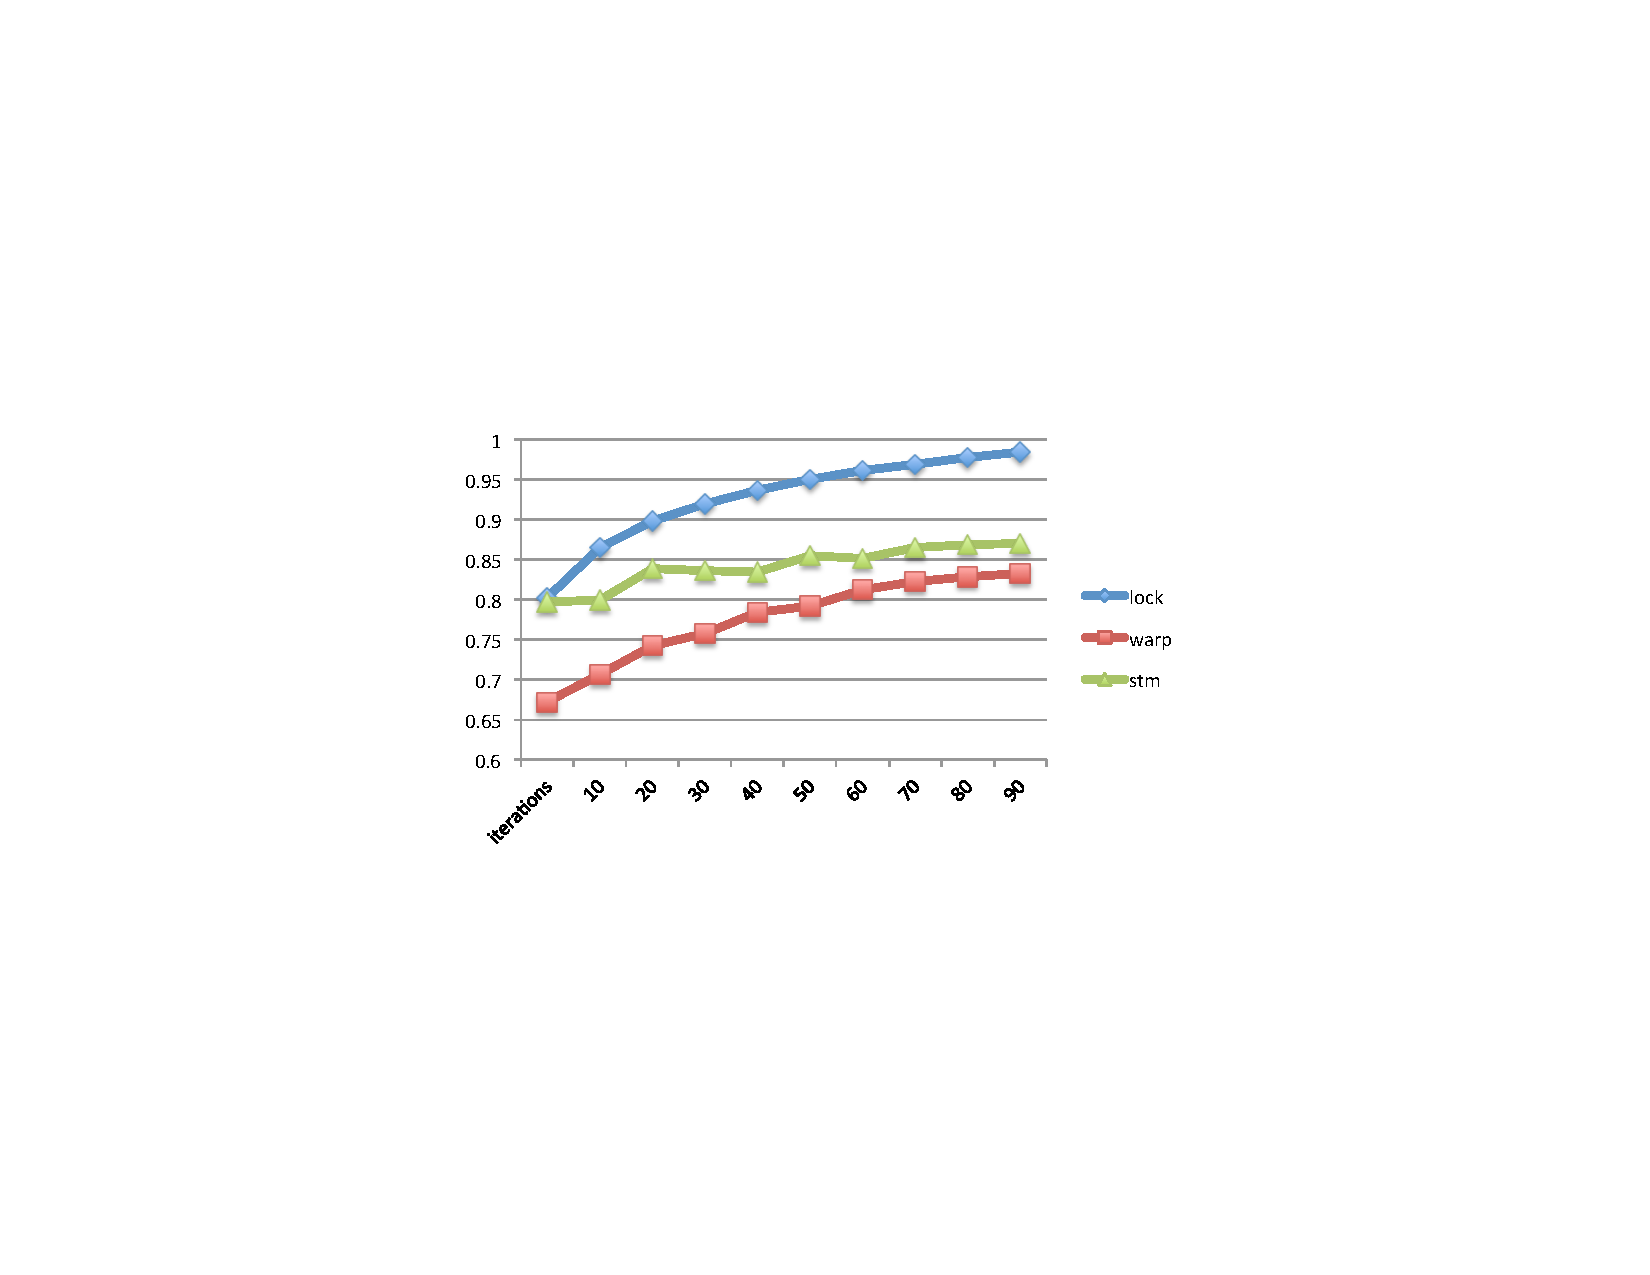
\includegraphics[width=\textwidth]{../../eval/32threads/case2it.pdf}
%		\caption{\label{Fi:case2it}dyuproject {\sf StandardConvertorCache}: workload}
%	\end{minipage}
%	\begin{minipage}{0.3 \textwidth}
%		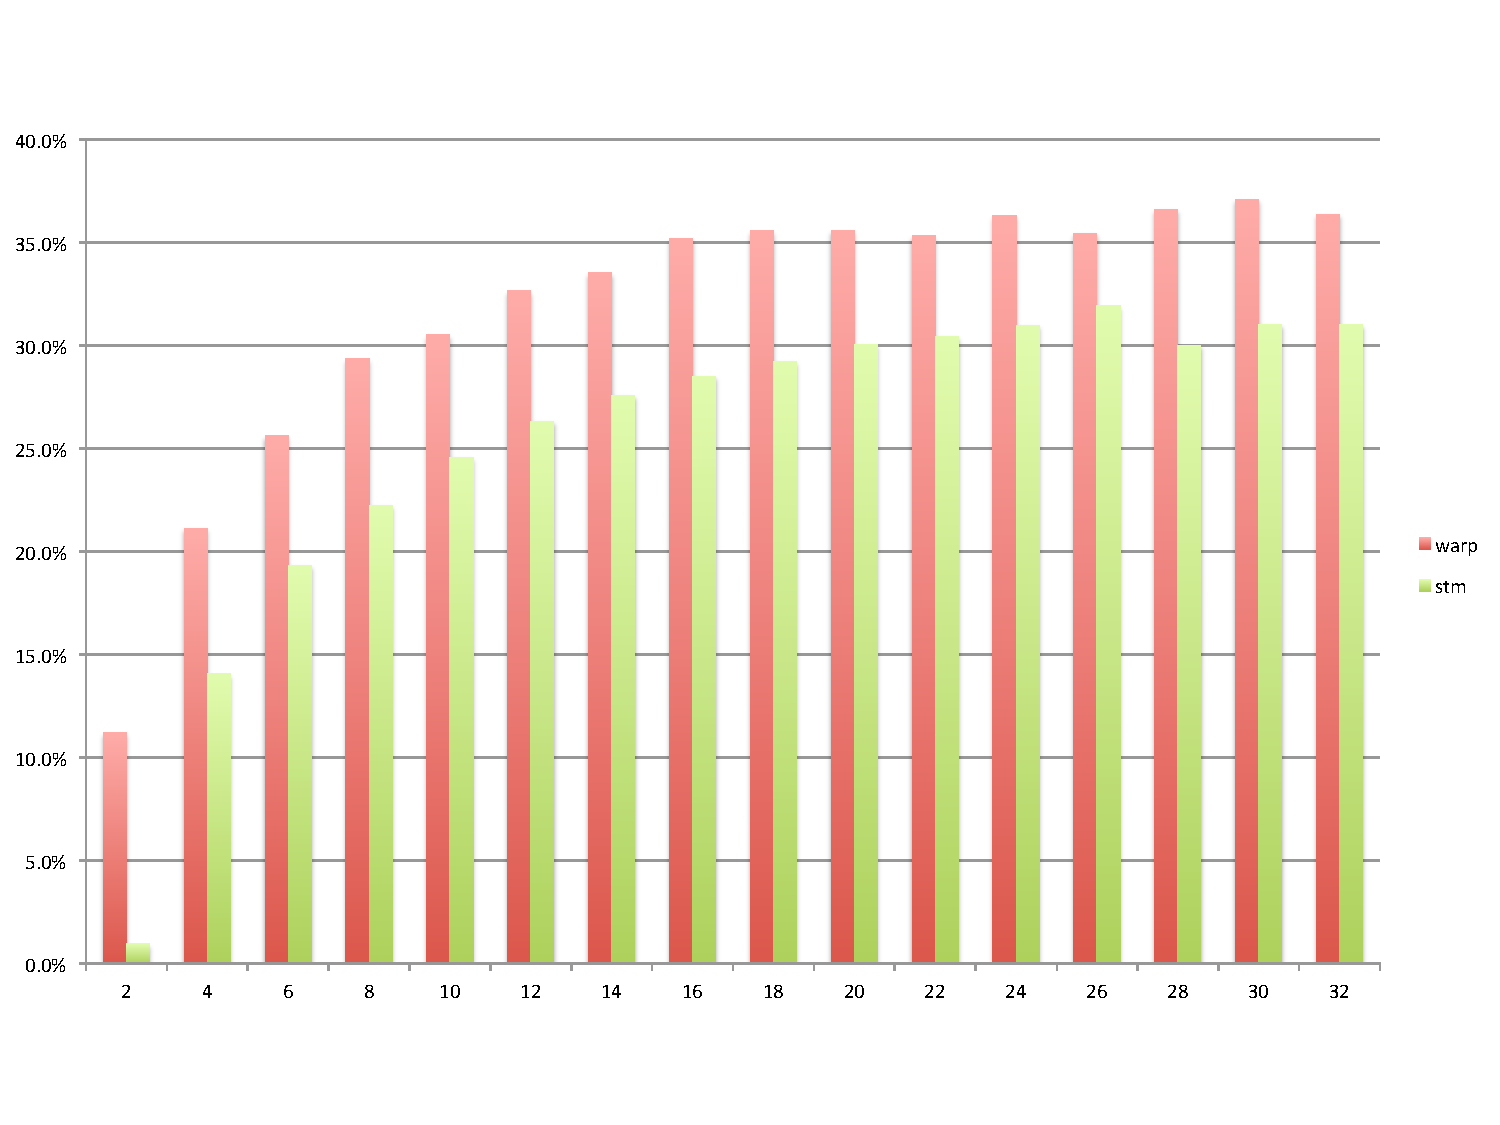
\includegraphics[width=\textwidth]{../../eval/32threads/case2th.pdf}
%		\caption{\label{Fi:case2th}dyuproject {\sf StandardConvertorCache}: concurrency}
%	\end{minipage}
%	\hspace{0.05 \textwidth}
%	\begin{minipage}{0.3 \textwidth}
%		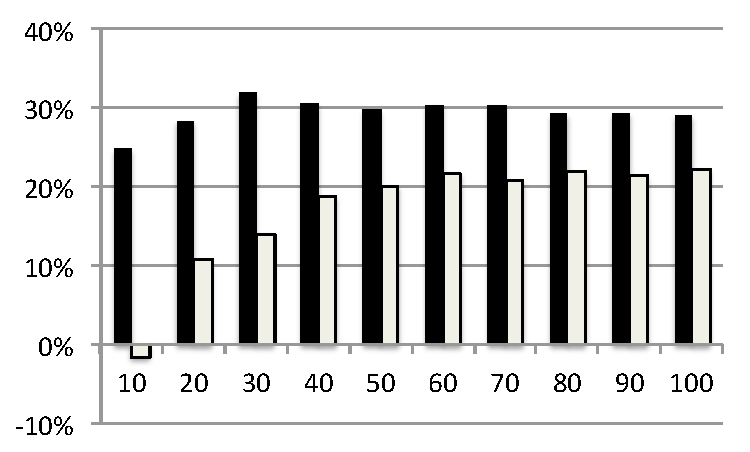
\includegraphics[width=\textwidth]{../../eval/32threads/case3it.pdf}
%		\caption{\label{Fi:case3it}Flexive {\sf FxValueRendererFactory}: workload}
%	\end{minipage}
%	\hspace{0.05 \textwidth}
%	\begin{minipage}{0.3 \textwidth}
%		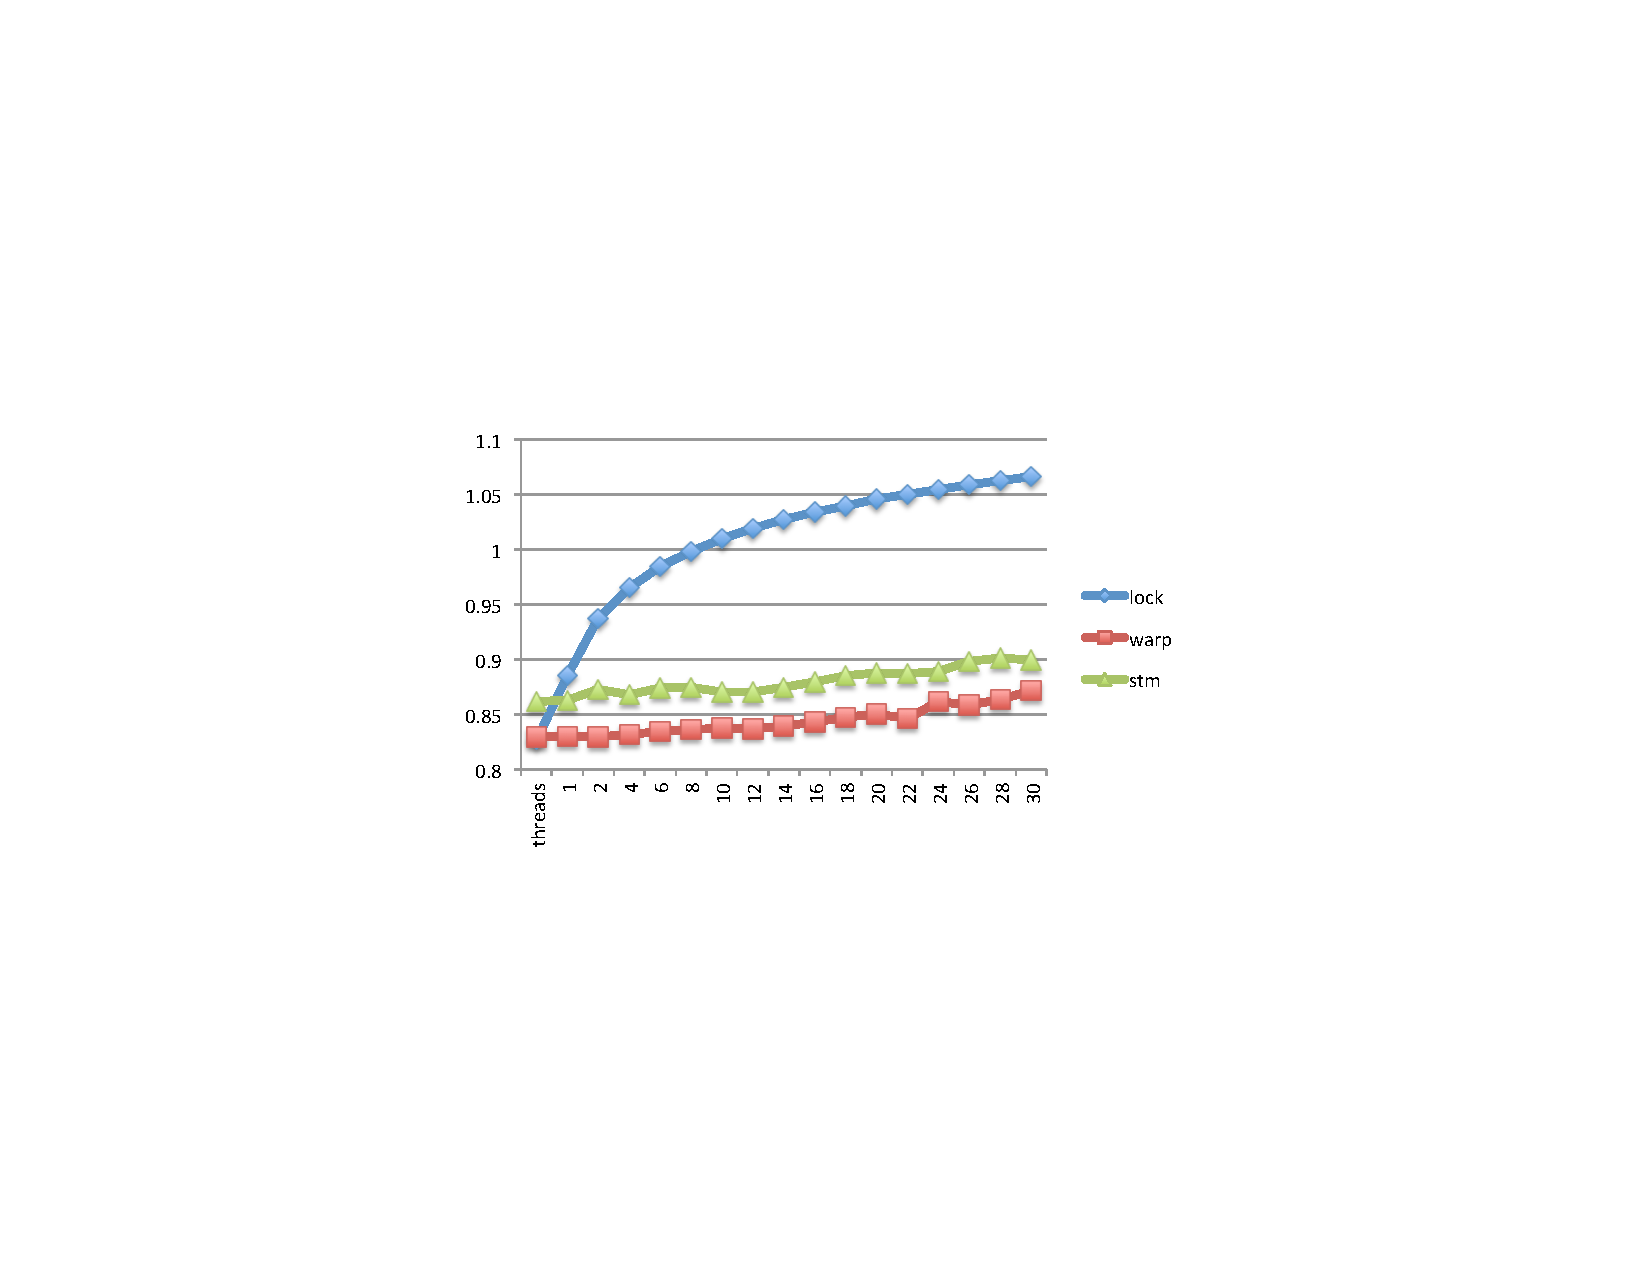
\includegraphics[width=\textwidth]{../../eval/32threads/case3th.pdf}
%		\caption{\label{Fi:case3th}Flexive {\sf FxValueRendererFactory}: concurrency}
%	\end{minipage}
%	\begin{minipage}{0.15 \textwidth}
%		\ 
%	\end{minipage}
%	\begin{minipage}{0.3 \textwidth}
%		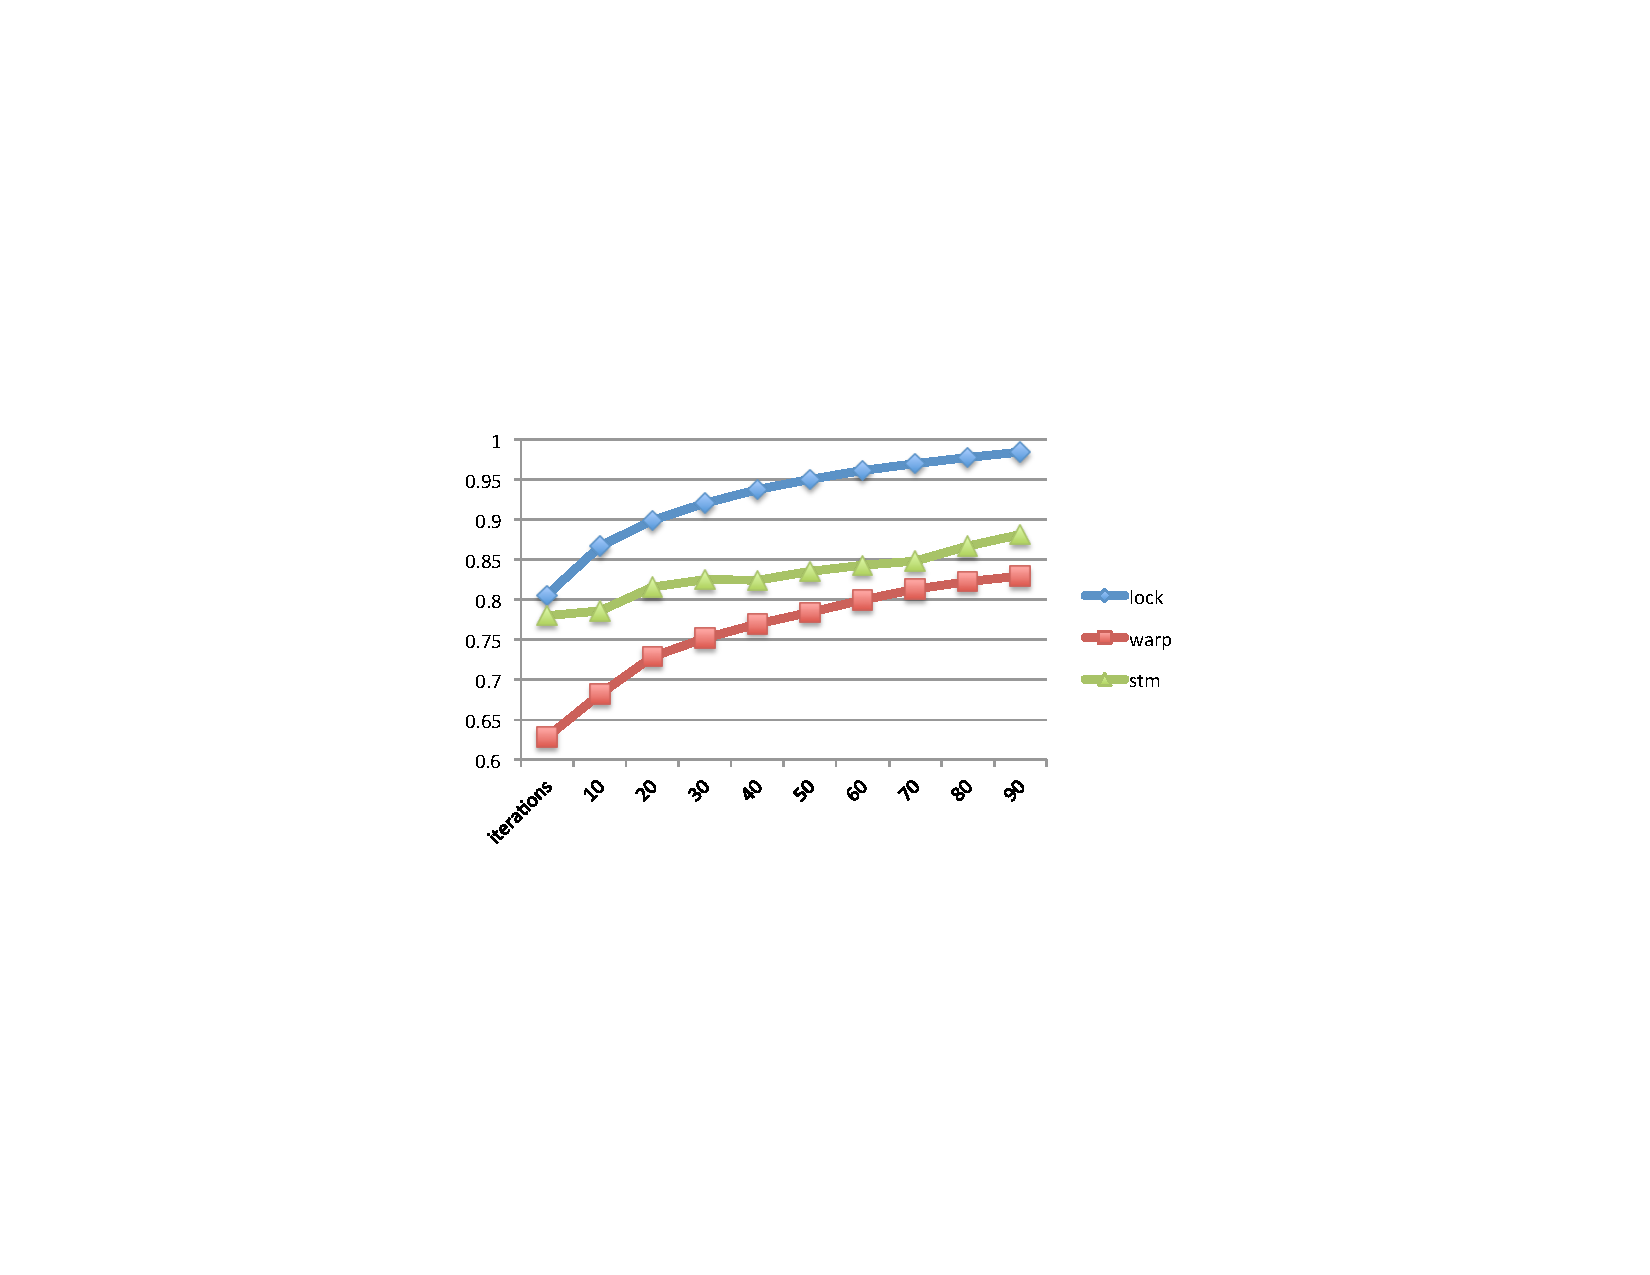
\includegraphics[width=\textwidth]{../../eval/32threads/case4it.pdf}
%		\caption{\label{Fi:case4it}Gridkit {\sf ReflectionPofSerializer}: workload}
%	\end{minipage}
%	\hspace{0.1 \textwidth}
%	\begin{minipage}{0.3 \textwidth}
%		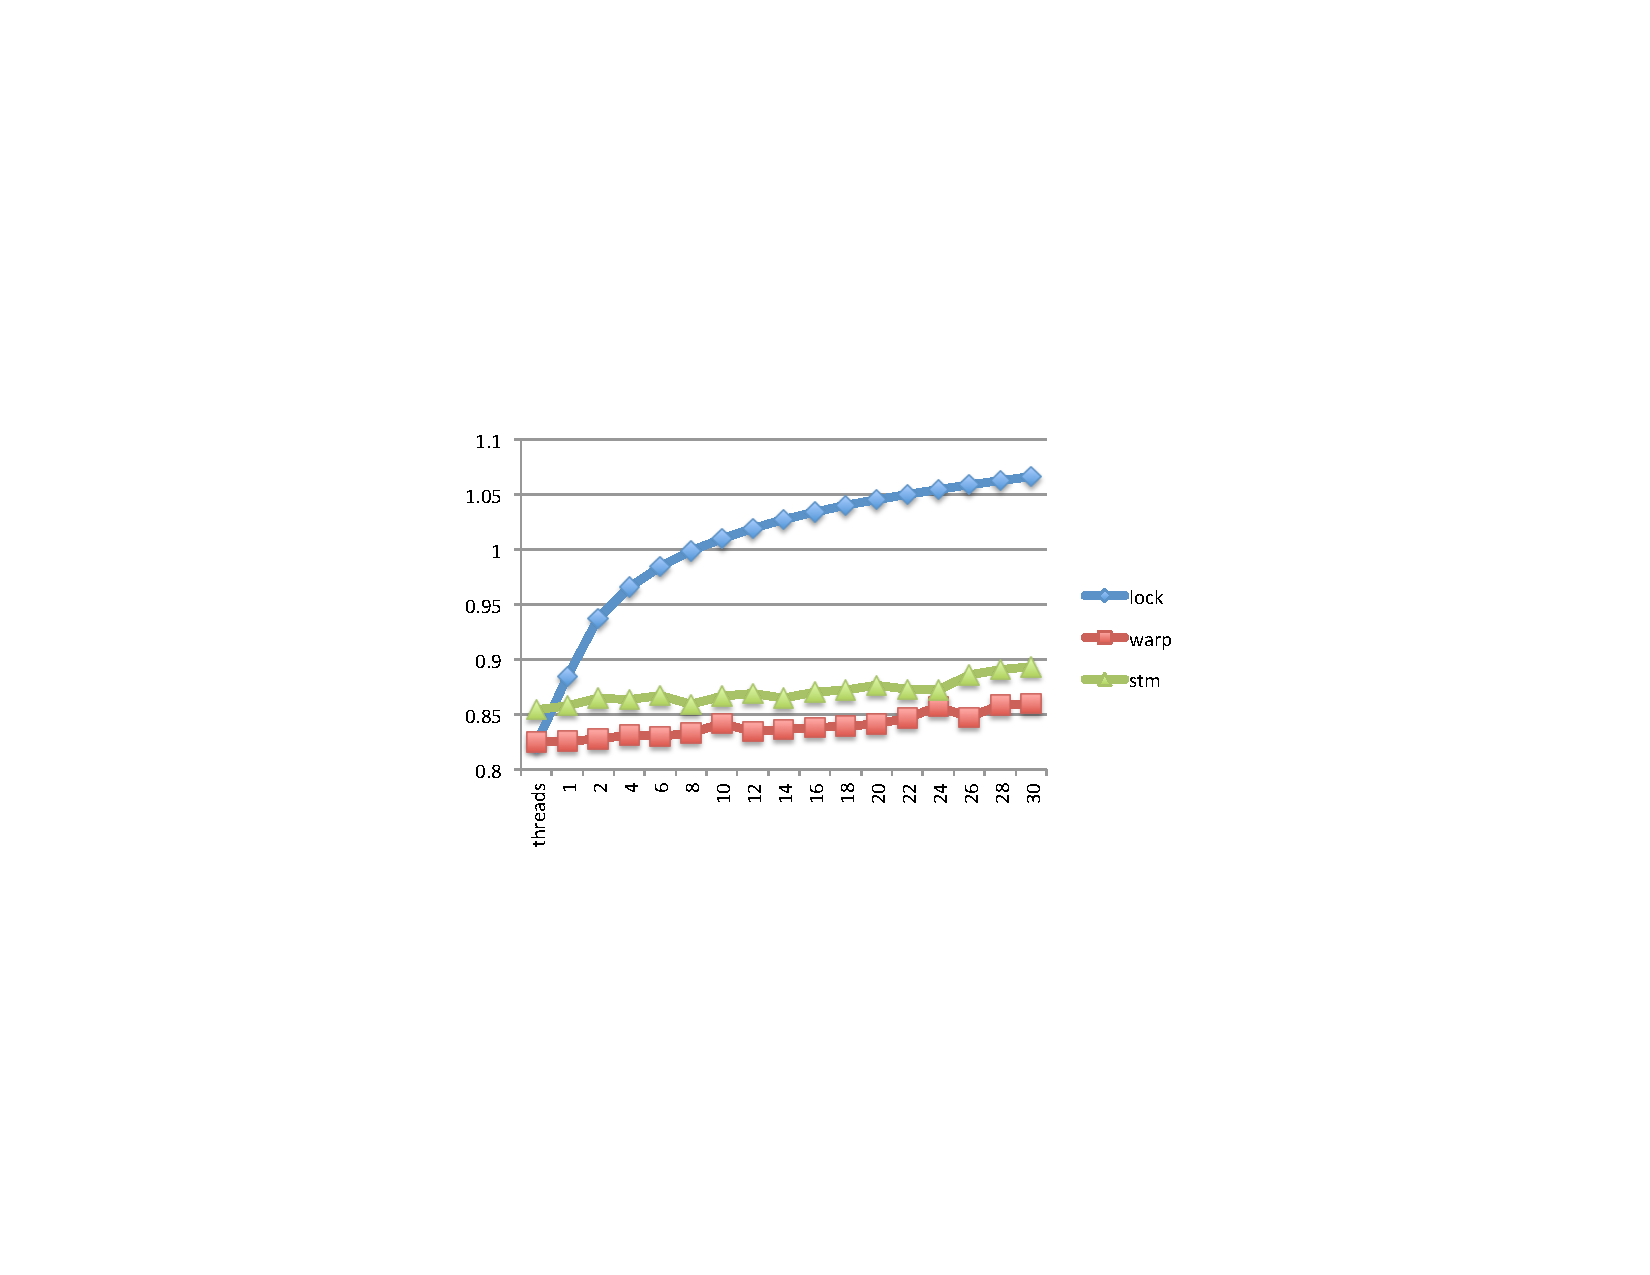
\includegraphics[width=\textwidth]{../../eval/32threads/case4th.pdf}
%		\caption{\label{Fi:case4th}Gridkit {\sf ReflectionPofSerializer}: concurrency}
%	\end{minipage}
\end{figure*}

\smartpar{Performance Results} 
%
We depict the performance results in Figures \ref{Fi:case1th}-\ref{Fi:case4th}, where for each benchmark we plot the results when increasing the size of the workload while fixing the number of threads (on the left), and when varying the number of threads (on the right).
Each plot presents a two column diagram, corresponding to STM and corrective synchronization (left/black and right/gray, respectively), which indicates the relative gain thanks to these approaches in comparison with lock-based synchronization. Indeed, the lock-based solution is overly conservative, yielding roughly a linear trend line of decrease in performance as either workload size or the number of threads increases.

%The left-hand-side charts correspond to the first measurement, where we increase the size of the workload while fixing the number of threads. The right-hand-side graphs correspond to a fixed-size workload executed by each of the transactions, where the number of threads is variable.

The aggregate performance results, averaging across all workloads and concurrency
\begin{wrapfigure}[10]{r}{0.50\textwidth}
\begin{tabular}{|l|c|c|c|c|}
\hline
  & \multicolumn{2}{c|}{STM} & \multicolumn{2}{c|}{corrective sync.} \\
					\cline{2-5} 
					& workload & conc. & workload & conc. \\
\hline
Tomcat	  	 &	1.5\%		&	3\% & 29\%		& 30\% \\			   
dyuproject	 & 	18\%		& 	24\%	    & 30\% &	29\%	\\
Flexive 		&	17\%	  &		14\%			& 29\% & 30\%	\\ 
Gridkit 		&	20\% 	&		16\%		& 32\% & 31\%	\\
\hline\hline	
{\bf average} & {\bf 14\%} 	&   {\bf 14\%}    & {\bf 30\%}   & {\bf 30\%} \\
\hline
\end{tabular}
%\end{center}
\end{wrapfigure}
levels, are summarized to the right.
For completeness, we also note the absolute running times, as min/max intervals in seconds, for the lock-based solution for the workload and concurrency configurations respectively: Tomcat -- [6,10], [7,12]; dyuproject -- [6,9], [7,11]; Flexive -- [6,10], [7,11]; and Gridkit -- [6,9], [7,11]. 
As the numbers indicate, corrective synchronization achieves better performance than STM with relative improvement on locks that is more than x2 better than STM.

\smartpar{Discussion}
%
An interesting observation w.r.t. the raw performance results is that while corrective synchronization provides stable and consistent performance improvement across all benchmarks, STM seems to do much worse on Tomcat compared to all other benchmarks. We have analyzed this gap.
%
The reason for this discrepancy,is that in both dyuproject and Flexive and Gridkit, once a first transaction manages to update the value corresponding to the input key, all other (nonoverlapping) transactions effectively become read-only transactions, and so conflict free. Hence STM achieves significant improvement compared to locks. In the case of Tomcat, however, this pattern does not hold. Transactions throughout the entire run perform write operations, leading to conflicts that degrade the performance of STM.

Interestingly, even on the benchmarks other than Tomcat STM is not able to compete with the low overhead, and thus better performance, of corrective synchronization. We suspect that the reason is that STM has to instrument memory accesses, whereas corrective synchronization applies state corrections directly.

%In Figure~\ref{fig:case2Iter}, the X axis is the number of transactions in each thread, Y axis is the running time (unit: milliseconds). We fix the number of threads as 8. Although the number of transactions changes, the ratio between the $lock/stm$ time and the $warp$ time remains around 5, i.e., the $warp$ version runs as  5X times as the $lock/stm$ versions. We interpret the results in the following ways. First, the $lock$ version essentially serialize all the transaction instances because they involve the same key. The $stm$ version also exhibits the  parallelism embarrassingly in this case: Many transaction instances unconditionally update the location of the key in the map, which conflict with the transaction instances that read the location and force them to rollback. The $stm$ and $lock$ versions have similar performance because they  both serialize the transaction instances. Second, the speedup of our approach over $lock/stm$ is fixed when the thread number is fixed, indicating that the speedup is subject to the number of threads. 
%
%
%
%In Figure~\ref{fig:case2Th}, the X axis is the number of threads, Y axis is the running time. We fix the number of transactions each thread runs as 100. The ratio between the $lock/stm$ time and the $warp$ increases when the number of threads increases. For example, the $lock/stm$ version takes around 2X time as the $warp$ with 2 threads, around 3X time with 4 threads, around 5X with 8 threads, and remain 5X with more than 8 threads. This observation confirms our previous conclusion that the speedup is subject to the the number of threads. In this case, we get the best the speedup with 8 threads, where 8 is also the number of the cores, indicating that we make full exploitation of the cores with 8 threads. The figure shows that our approach has the dramatically better thread scalability than existing approaches. Another interesting observation is, when there is a single thread, the stm version takes 164 ms, while both our version and the lock version takes 112 ms. The stm takes longer time because the Deuce implementation instruments the classes on  the fly when they are loaded, which consumes extra time. 
%
%
%Figure~\ref{fig:case3Iter}, Figure~\ref{fig:case4Iter} and Figure~\ref{fig:case4Iter} show the performance when the workload increases and follow the same setting as the test 2 shown in Figure~\ref{fig:case2Iter}. Similar to Figure~\ref{fig:case2Th}, Figure~\ref{fig:case3Th}, Figure~\ref{fig:case4Iter} and Figure~\ref{fig:case4Iter} show the performance when the number of threads increases. From the figures, we see the trend of the lock version and our version resemble case 2, but the stm version behaves quite differently. An interesting observation is, the time difference between the stm version and ours is almost a constant. This suggests that the stm version achieves the same parallelism degree as ours, while incurring some extra  overhead of class instrumentation. We inspected the code and confirmed this conclusion. In these cases, many transaction instances first check and then update conditionally. After the first instances update, the following instances will fail the checking and are degenerated to read-only transactions. The read-only transactions allow the maximal parallelism like ours. 
%
%\subsection{Discussion}
%
%{\bf Execution Summary\ } The static analysis phase computes a set of execution summaries, each representing a legal execution, which are used as the input of the dynamic analysis phase.
%Each execution summary describes (i) the return value of each transaction instance and (ii) the final map state
% 
%
%In our experiments,  we have two threads running two types of transactions ($TX_1$ and $TX_2$) respectively. One exemplary execution summary is, $[key\rightarrow v^1_1, r^1_1:v^1_1, r^n_1:v^1_1, r^1_2:v^1_1, r^n_2:v^1_1]$, where $r^1_1$ is the symbolic form of the return value of $TX^1_1$ (1$st$ instance of $TX_1$), $v^1_1$ is the symbolic form of the value put by the transaction instance, and $r^1_1:v^1_1$ describes the return value of the transaction instance. The readers may notice $r^n_1$. This symbol represents the return value of the instances that are not explicitly specified.  Here $n$ is determined by the capability of the static analysis. At runtime, we track the instance order and use $n$ by default if the number is not specified in the summary. The tracking of the instance order requires us to synchronize the first $n-1$ instances. However, the $n$ is typically a small number, and the synchronization overhead is negligible. We do not need to synchronize starting from the $n$th instance because all these instances are represented as $n$ by default. In addition, $key\rightarrow v^1_1$ tells what the key is associated with in the final map state. 
%
%The execution summary is not limited to the above basic case. In general, it is initial-state sensitive, schedule-oblivious and site-sensitive. 
%First, the initial state about whether the key is mapped to some value affects the computation of the execution summaries. Therefore, we prefix each execution summary with a specific initial state, e.g., the state with initial key $[key^{init}\rightarrow v^{init}]$ or the state without initial key $[key^{init}\rightarrow void]$.
%Second, our execution summary is designed to be oblivious of the schedules. The schedule-obliviousness frees us from tracking the schedules at runtime and avoids the high tracking overhead. Third, the execution summary is site-sensitive. A transaction $TX^1_1$ may put a value dynamically created at site $A$ to the map. We symbolically represent the value using the site and the occurrence of the site (inside the transaction instance), e.g., $A1$ in $TX^1_1$. The extent to which we can distinguish the occurrences is determined by the static analysis, e.g., how many iterations can be unrolled.
%
%
%{\bf Runtime System\ }
%The runtime works as follows. We first use the counters to track the transaction instance and assemble the symbolic return accordingly, e.g., $r^1_1$.
%Then we search for the symbolic value in the execution summaries, e.g., $v^1_1$. Last, using the symbolic value as a key, we look up the cache, which is maintained to associate each symbolic value with a runtime value, for the concrete runtime value.
%
%The second step, i.e., searching for symbolic value in the summaries, is challenging. The searching is demanded on the fly at the return of each transaction instance. 
%However, the returns should be consistent with each other such that the warped execution represents a realistic execution. In the other words, the return values should be searched for in the same execution summary. To achieve this, we implement an on-the-fly pruning algorithm. At the first return, it finds the symbolic value in a randomly picked execution summary. After the value is picked, the execution summaries with different value for the return will be pruned, leading to a smaller solution space. 
%The algorithm is iteratively applied. In addition, to achieve initial-state sensitivity, we also reduce the solution space based on the initial states. 
%
%Another tricky issue is, at some return, the symbolic value found in the execution summaries may have not been associated with any concrete runtime value yet.
%For example, at the return of $TX^1_2$, we find the returned value as $v^1_1$ but $TX^1_1$ has not been executed, then we cannot find the runtime value associated with $v^1_1$ in the cache. This case happens because the execution summary is computed for certain schedule, which differs from the current schedule. In this case, we apply the notify/wait primitives to synchronize the cache lookup and cache maintenance. Even more complex, the returned value may never be put into the cache if the value creation site is disabled in the current schedule, e.g., its guarding branch condition is false. We simply remove all the guarding branches for the creation site such that it is always executed. This simple strategy is based on the insight that we treat the transaction as a blackbox and we only care about its return values. It is unnecessary to preserve the internal program semantics.
%
%
%We also implemented the optimization for the caching. From the summaries, we see that only the values put by the first few transactions are used. Therefore, we only record such values into the cache and discard the rest at runtime.
%
%
%
%
%
%
%\subsection{Evaluation}
%
%%TODO: check if we need to remove teh business op from the warp version.
%For performance measurement, we compare 4 versions with different types of synchronizations, the original version $orig$, the abstract key locking version $key$, the software transactional memory version $stm$, and the warping version $warp$.  The original version is without any synchronization, which may produce incorrect outputs. 
%We use this version to approximate the best performance any synchronization can achieve. The abstract key locking protects each key with a unique lock~\cite{}. As compared to protecting the whole map with a single lock, it allows parallelism among the invocations with different keys. For the software transactional memory, we use the open sourced implementation {\sf Deuce}~\cite{}. {\sf Deuce} features the easiness of use. {\sf Deuce} is essentially a Java agent that instruments the classes during the class loading to insert the STM functionality. However, the JDK classes are loaded before the agent starts to work. Therefore, we re-import the JDK implementation as application classes, which {\sf Deuce} successfully apply to. 
%The $warp$ version adopts our algorithm. In our evaluation, we use both the initial state with the key and the initial state without the key.  For space reason and clarity of figure, we only show the result based on the initial state with the key (other results are put into the technique report).
%
%
%Our benchmark is adapted from real world applications, including XXX and YYY. In our experiment, we consider two types of transactions for each benchmark, and each thread runs a combination of the transactions. In our experiment, we measure the performance under two changes: (1) We fix the number of threads as 8, the number of cores in the machine, and then change the number of transactions each thread runs from 10 to 100. This setting helps us understand the performance in different workloads, (2) we fix the number of transactions each thread runs as 100, and change the number of threads following the sequence: 1,2,4,6,8,10,12,14,16. This setting allows us to study the thread scalability. In our experiments, all threads operate on the same key.

%\begin{figure*}
%\centering
%\subfloat[{Case 2 with the increasing workload}]{\label{fig:case2Iter}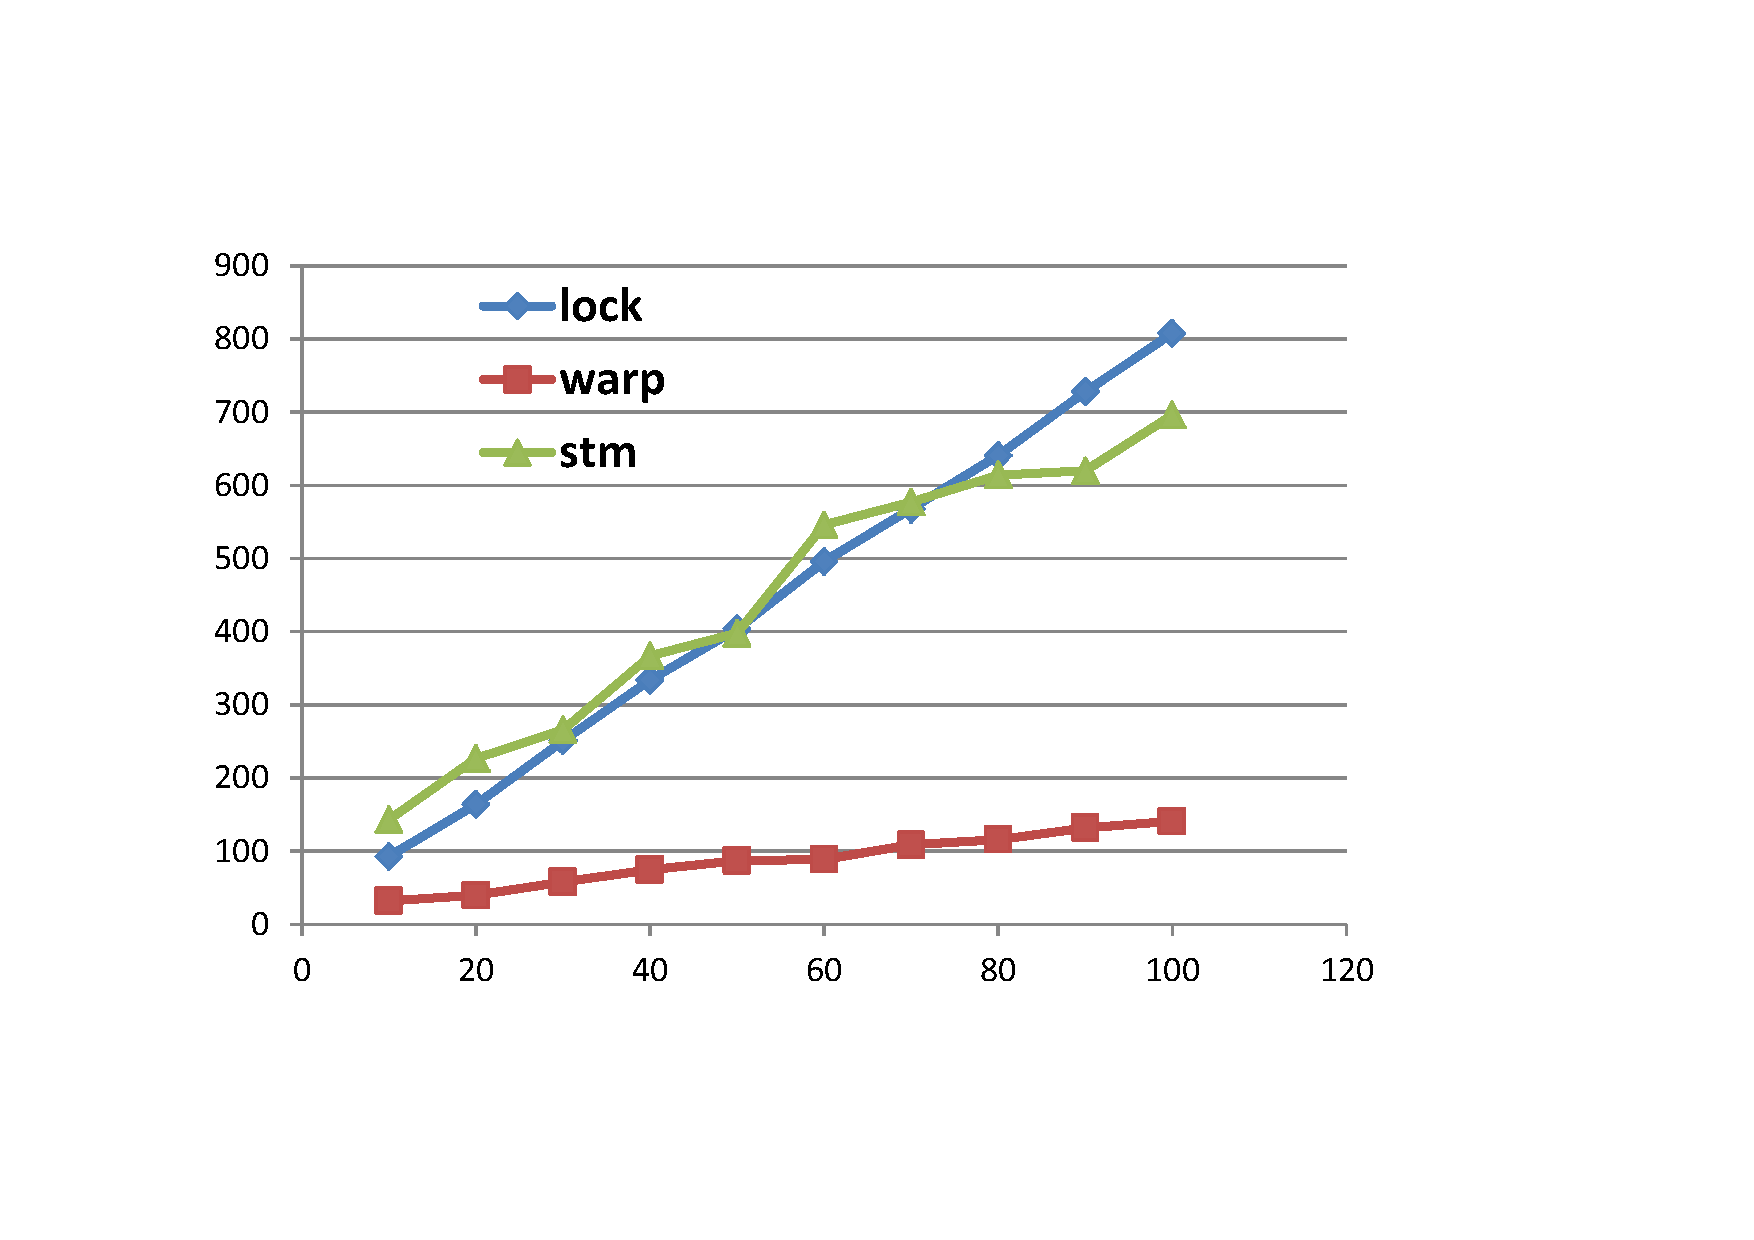
\includegraphics[width=0.33\textwidth]{../../eval/case2-varyIter.pdf}}
%\subfloat[{Case 2 with the increasing number of threads}]{\label{fig:case2Th}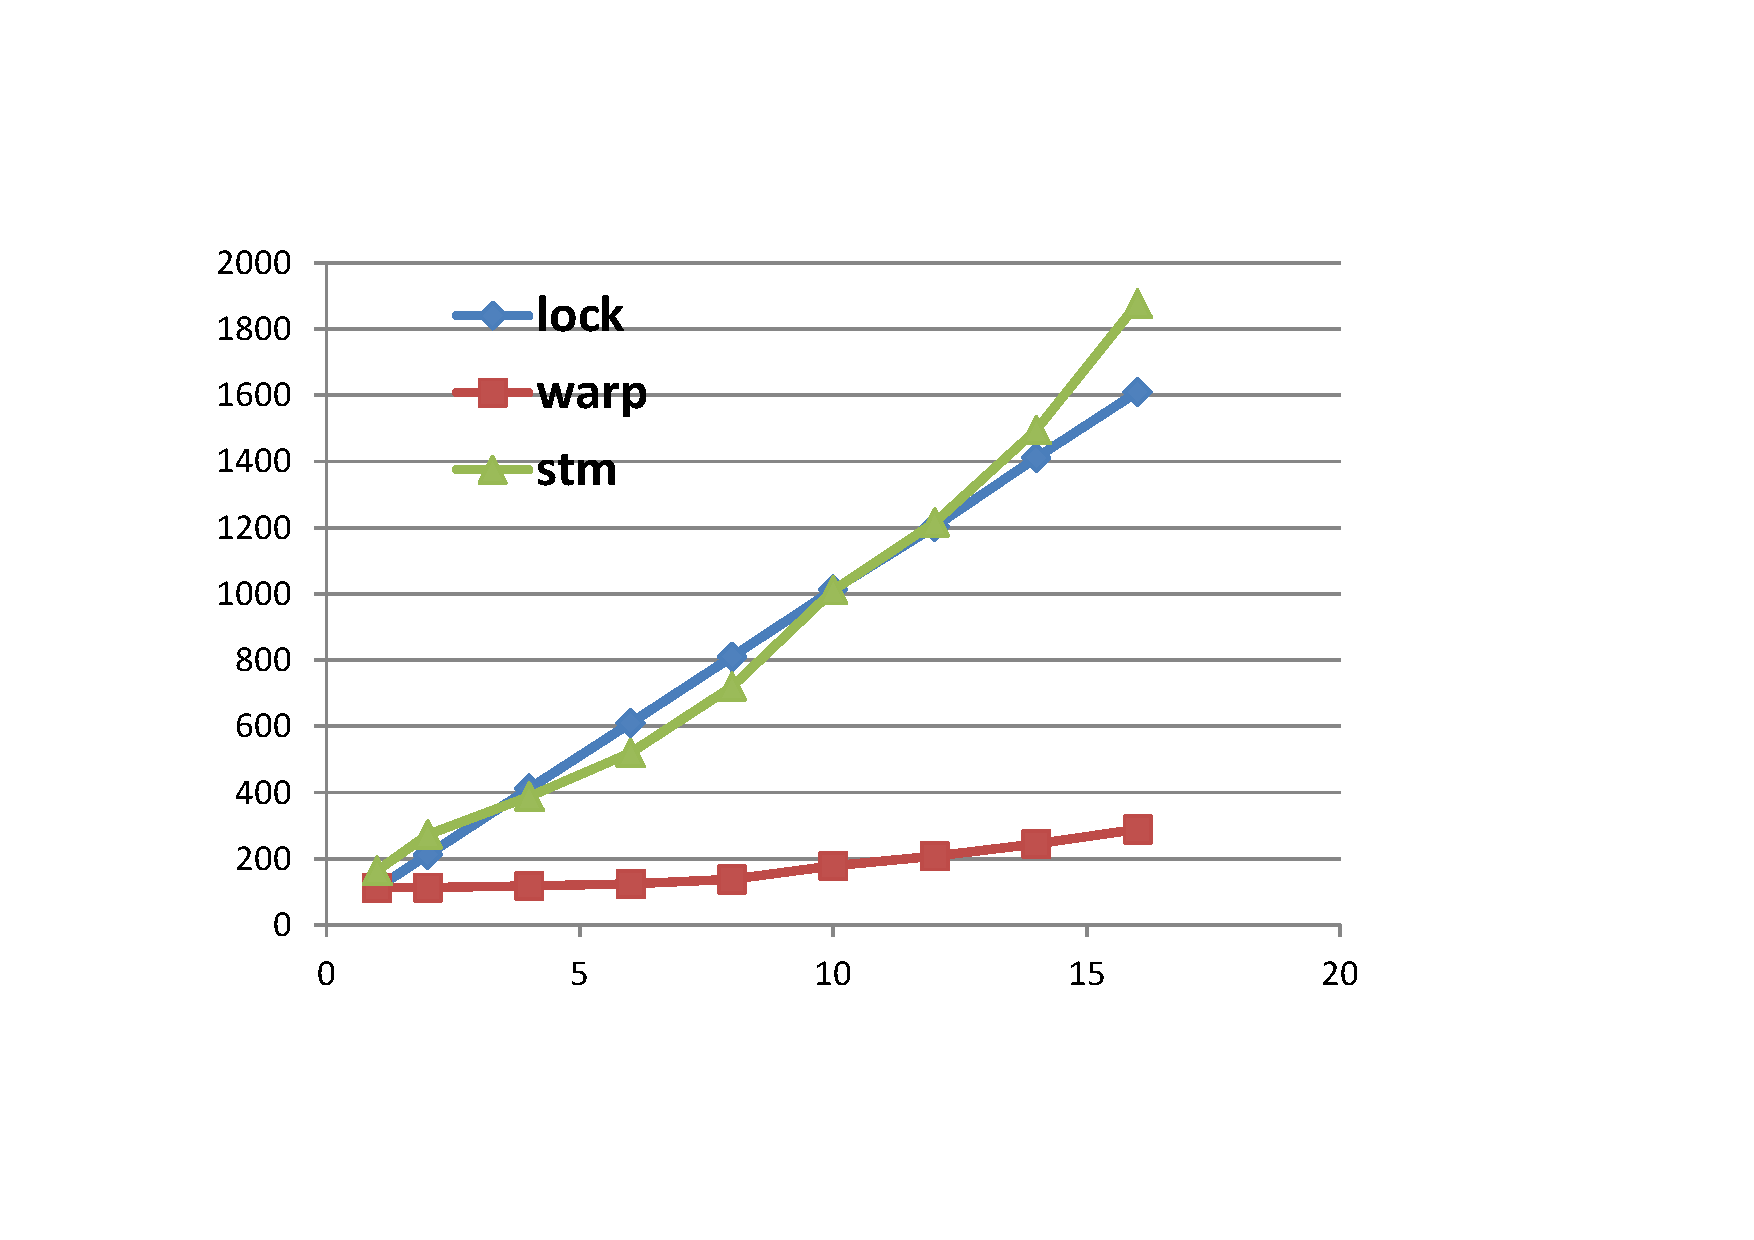
\includegraphics[width=0.33\textwidth]{../../eval/case2-varyThreads.pdf}}
%\\
%\subfloat[{Case 3 with the increasing workload}]{\label{fig:case3Iter}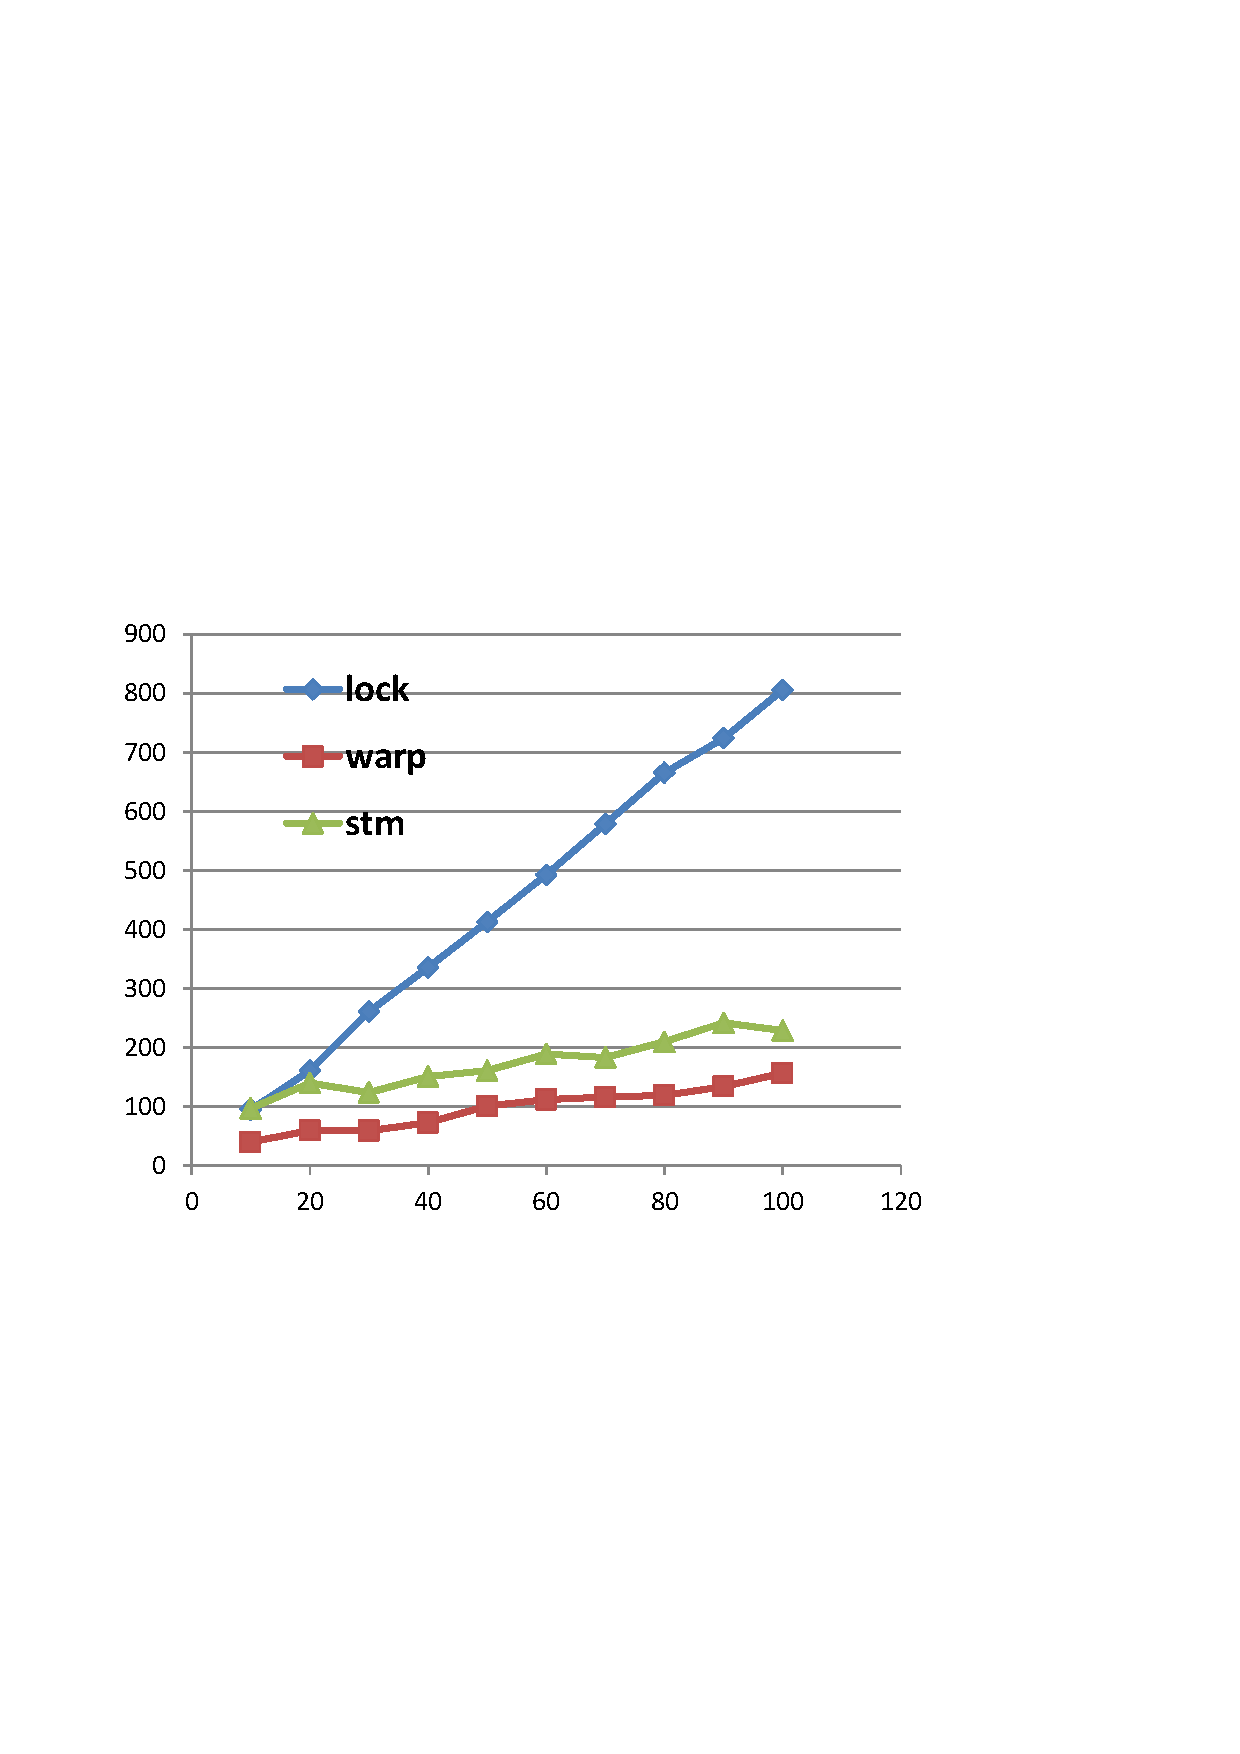
\includegraphics[width=0.33\textwidth]{../../eval/case3-varyIter.pdf}}
%\subfloat[{Case 3 with the increasing number of threads}]{\label{fig:case3Th}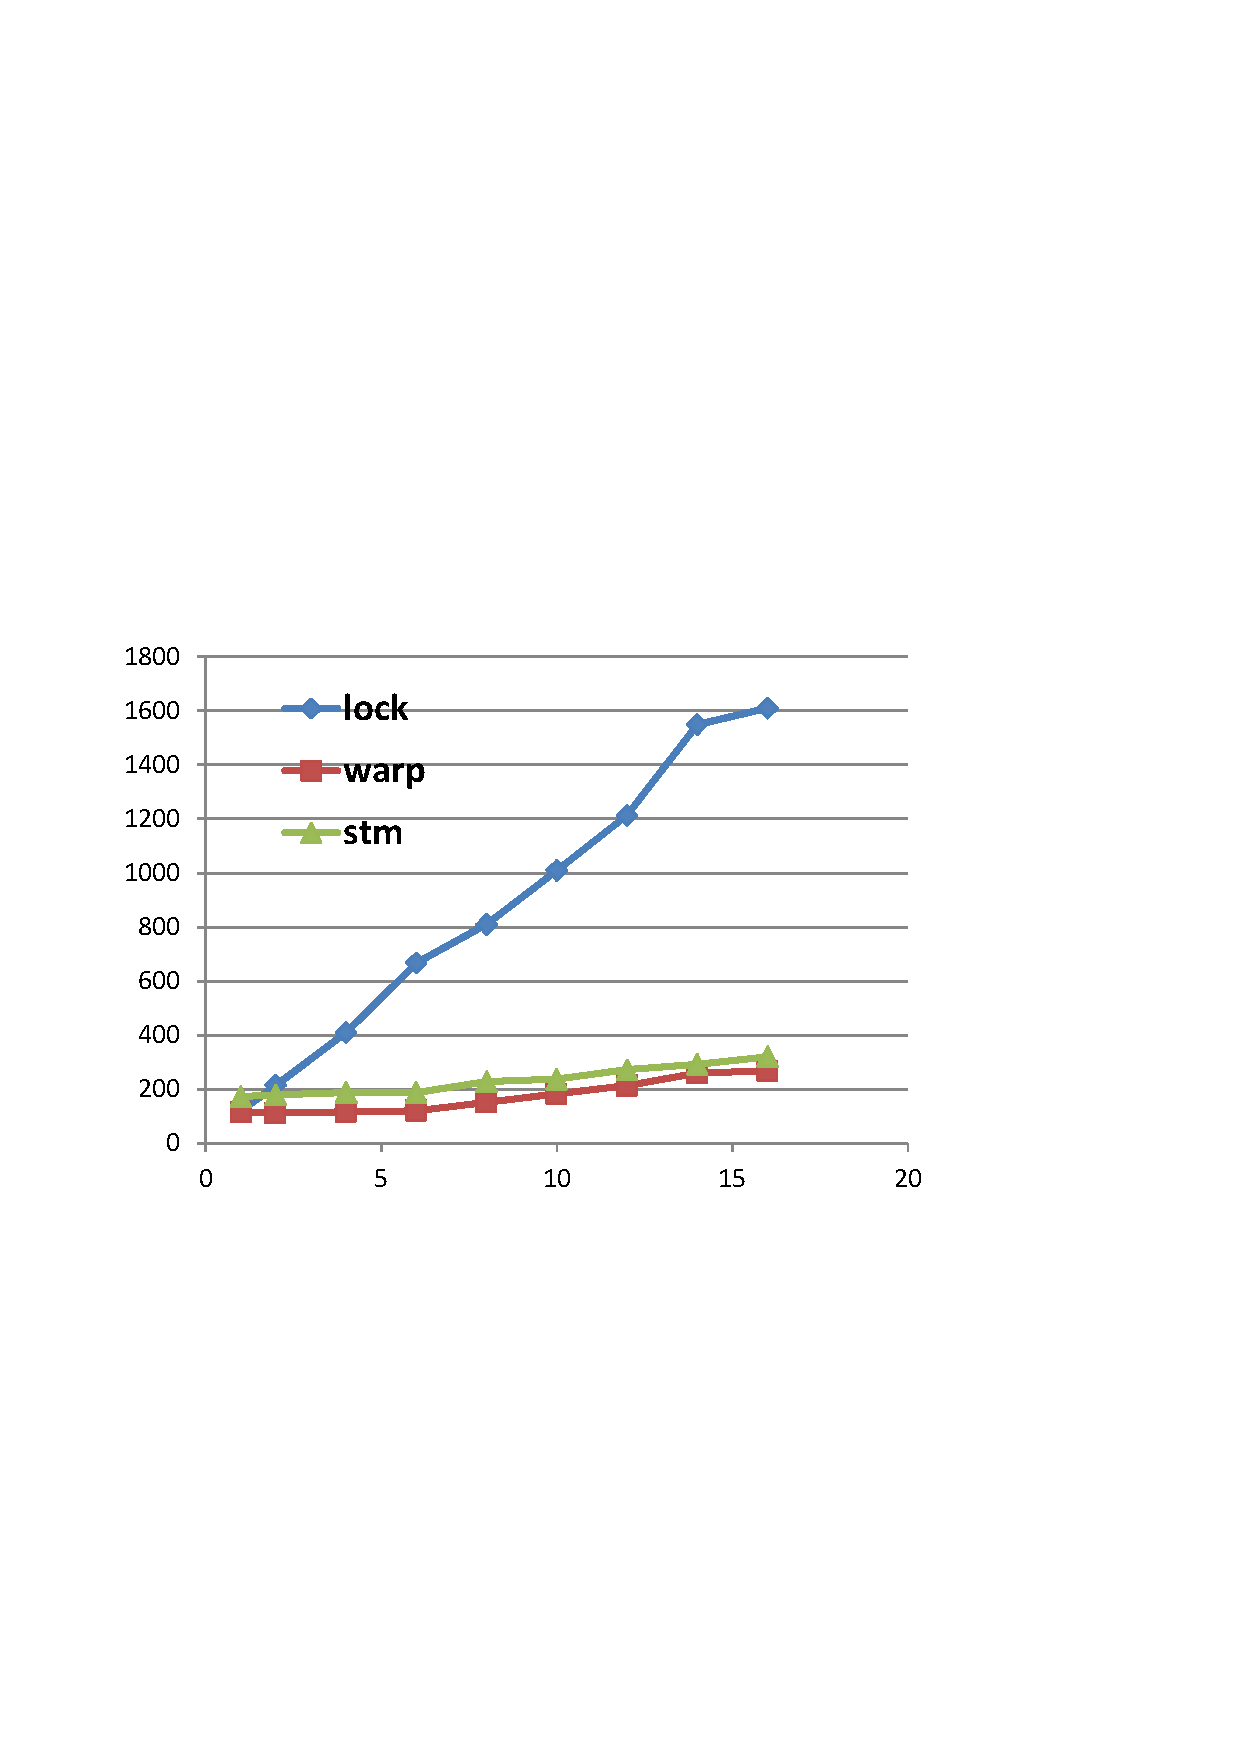
\includegraphics[width=0.33\textwidth]{../../eval/case3-varyThreads.pdf}}
%\\
%\subfloat[{Case 4 with the increasing workload}]{\label{fig:case4Iter}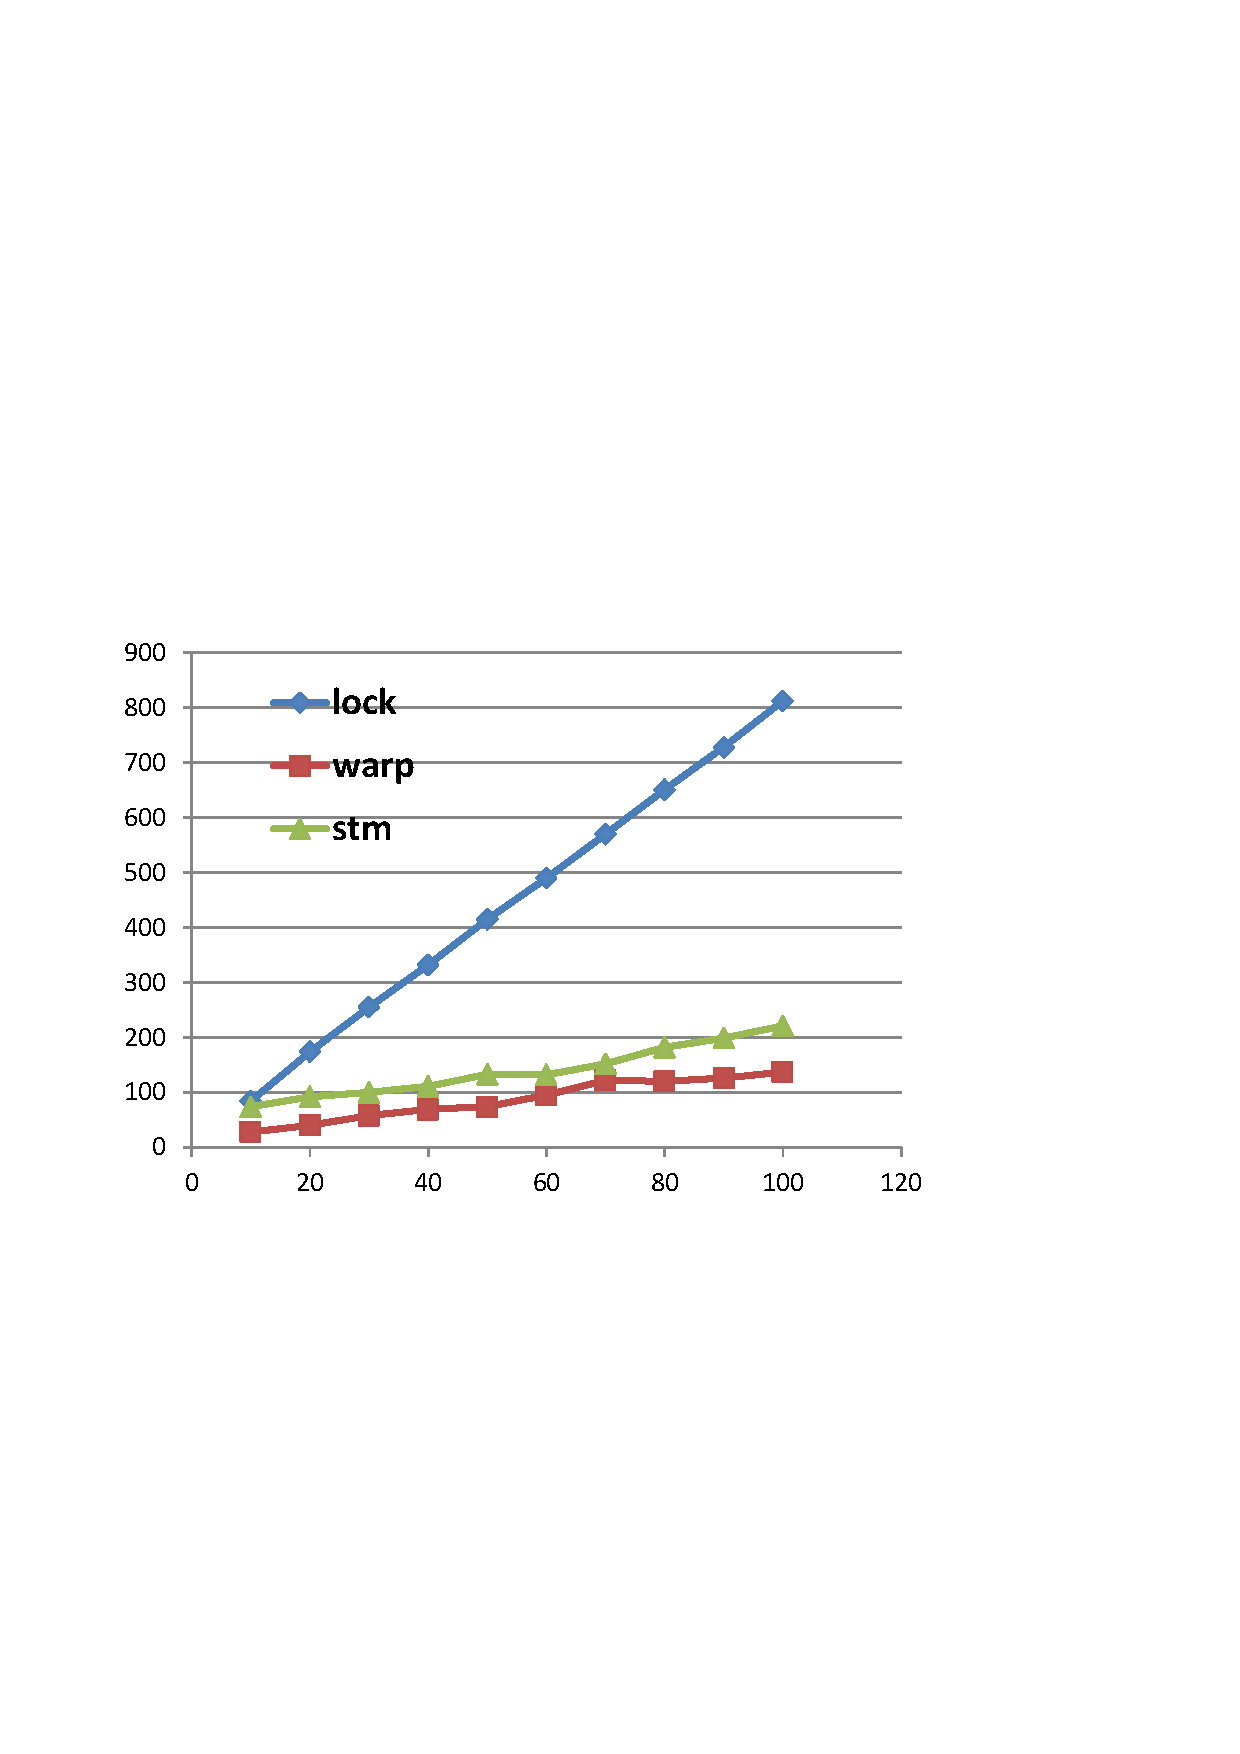
\includegraphics[width=0.33\textwidth]{../../eval/case4-varyIter.pdf}}
%\subfloat[{Case 4 with the increasing number of threads}]{\label{fig:case4Th}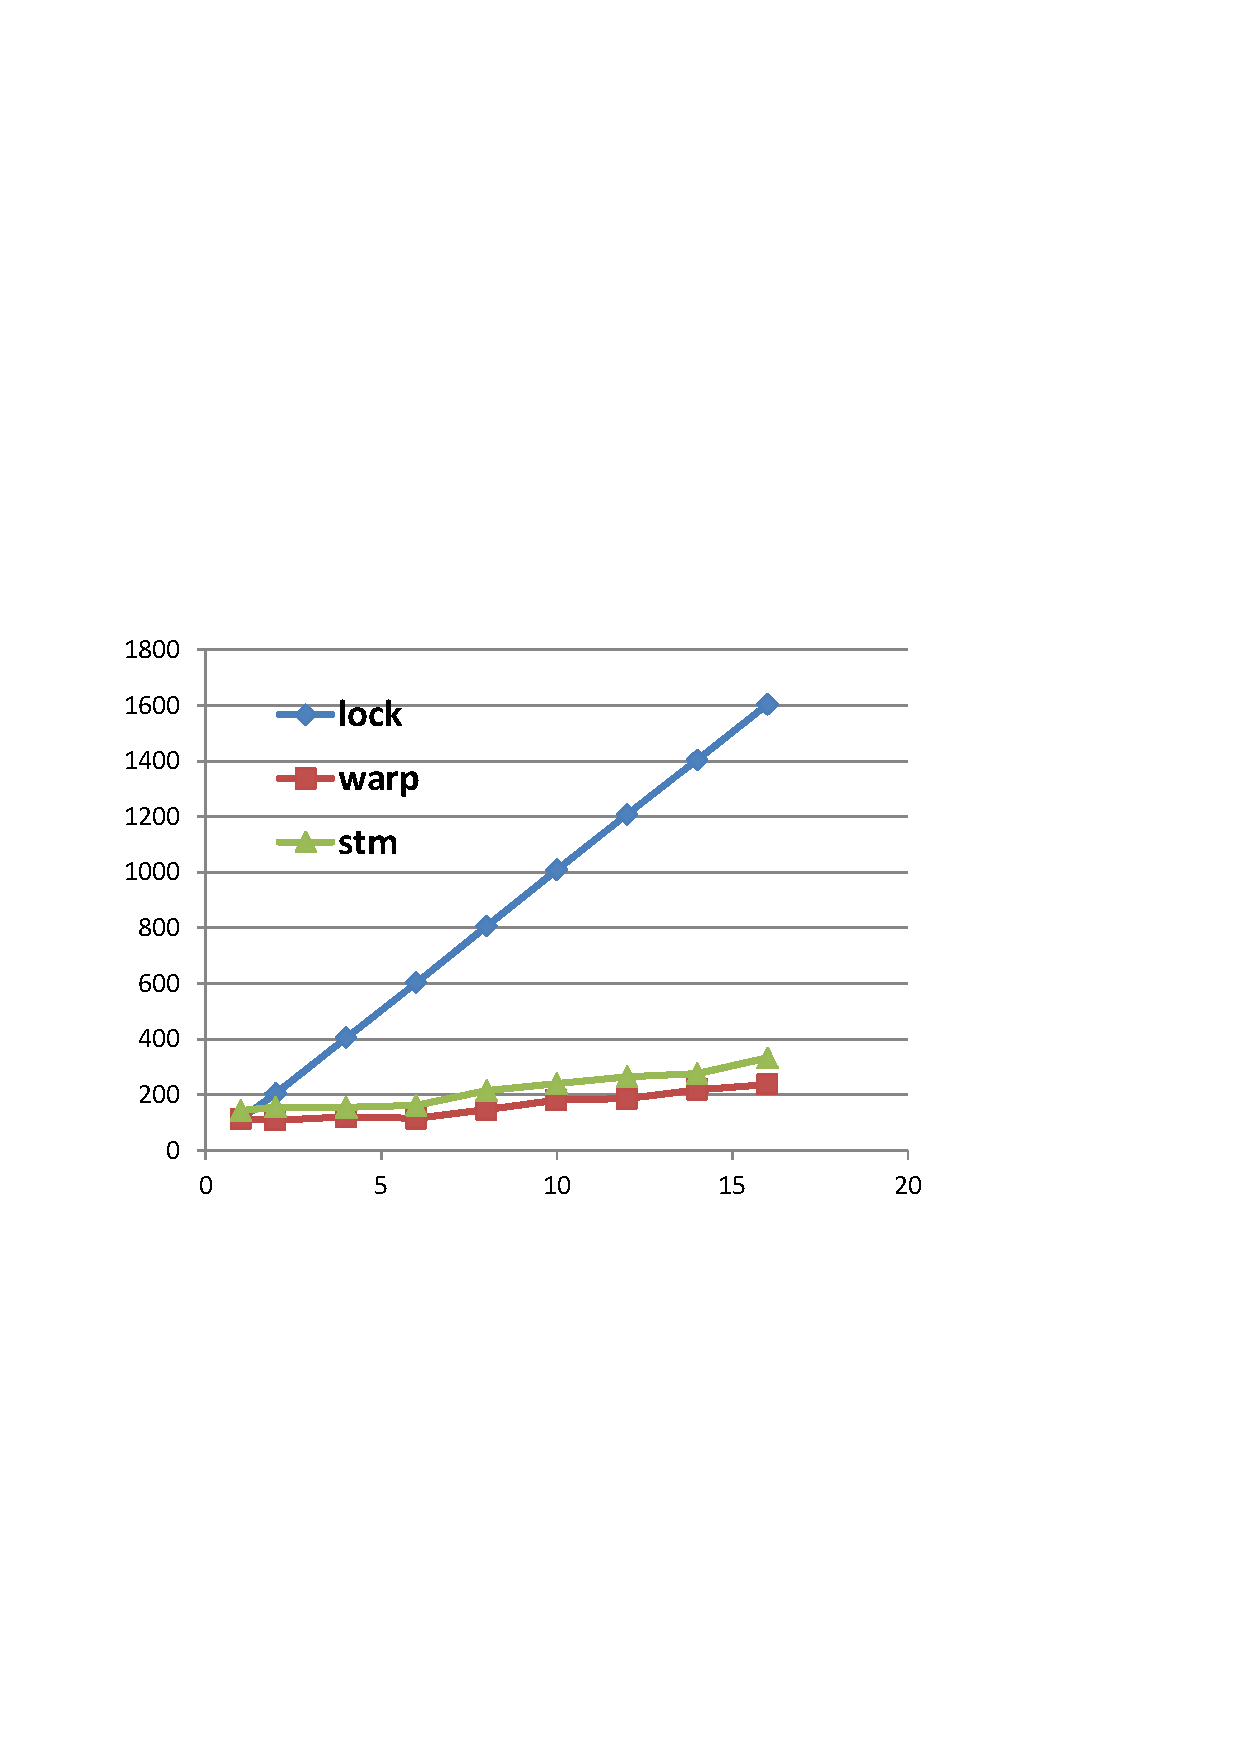
\includegraphics[width=0.33\textwidth]{../../eval/case4-varyThreads.pdf}}
%\\
%\subfloat[{Case 5 with the increasing workload}]{\label{fig:case5Iter}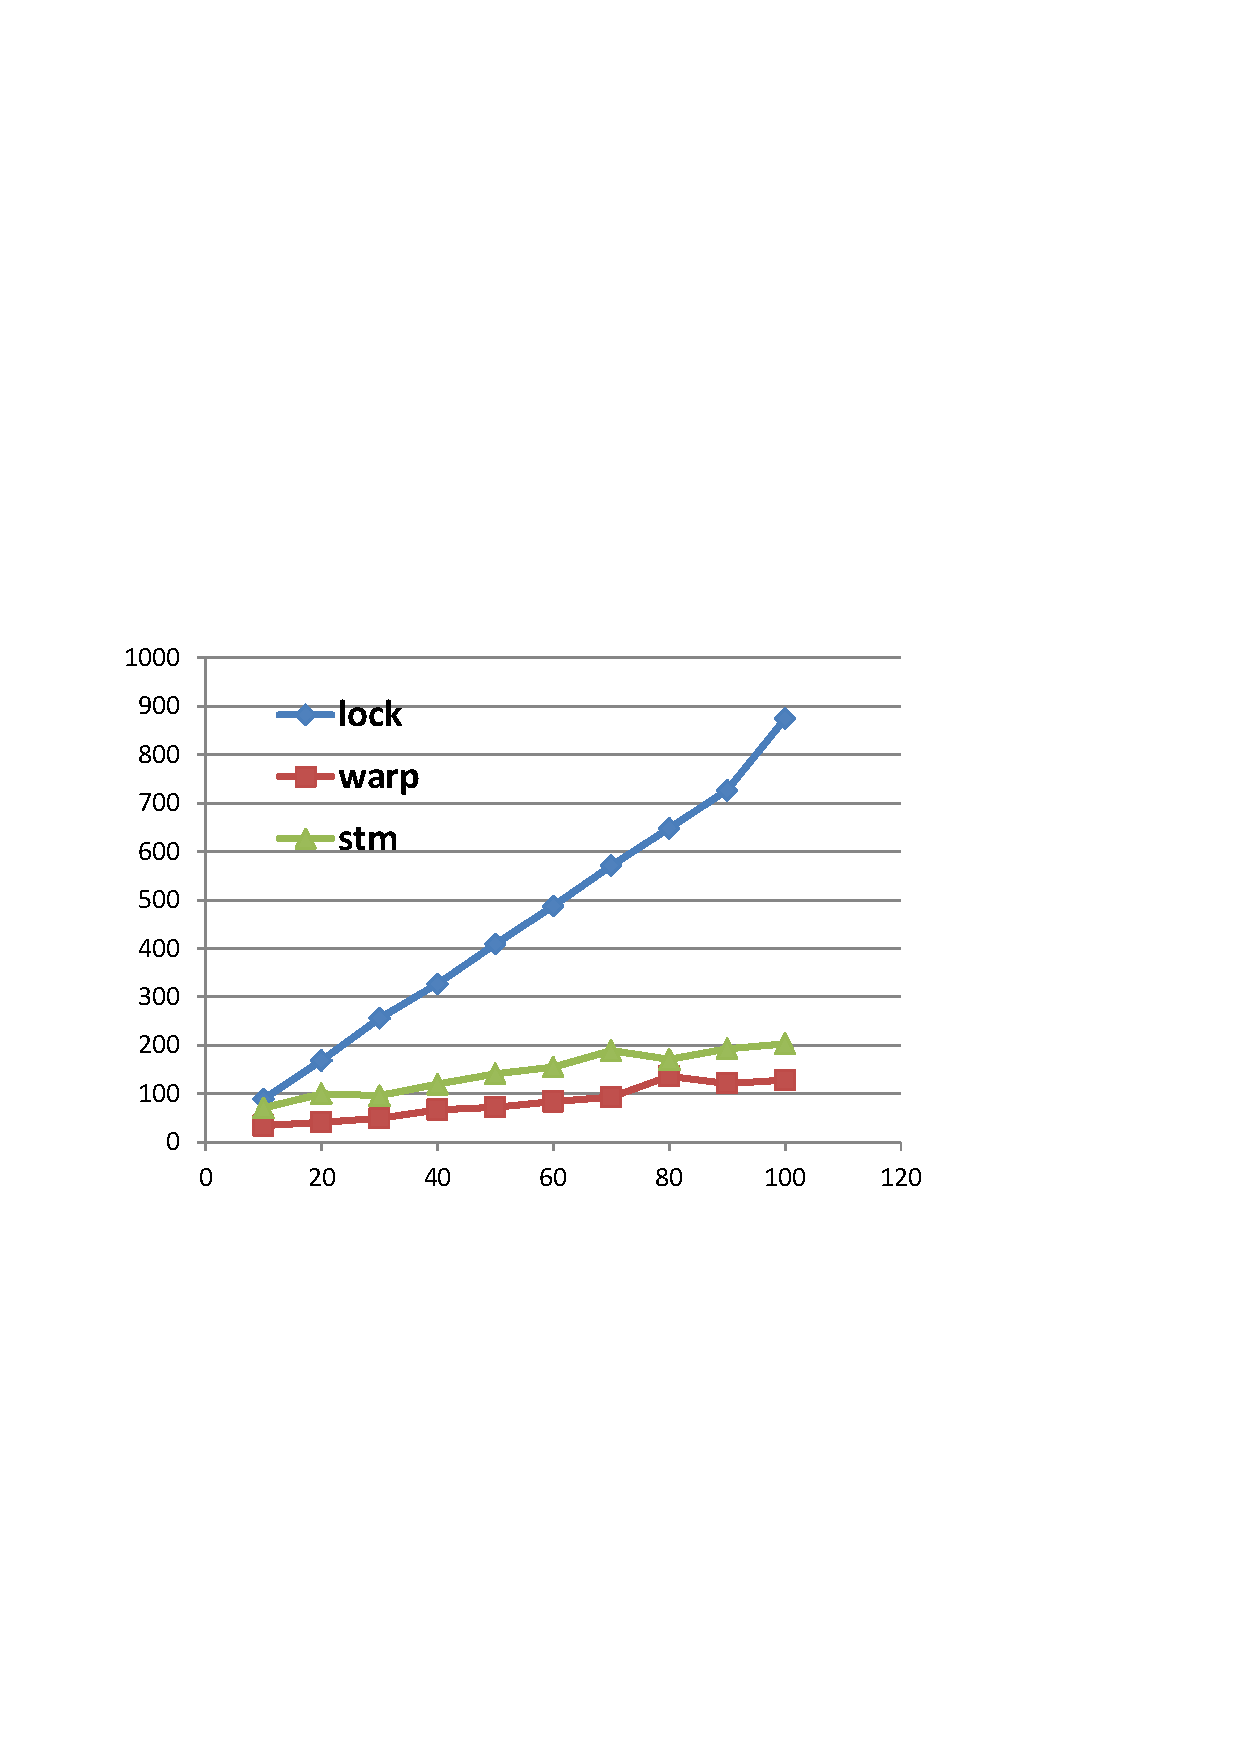
\includegraphics[width=0.33\textwidth]{../../eval/case5-varyIter.pdf}}
%\subfloat[{Case 5 with the increasing number of threads}]{\label{fig:case5Th}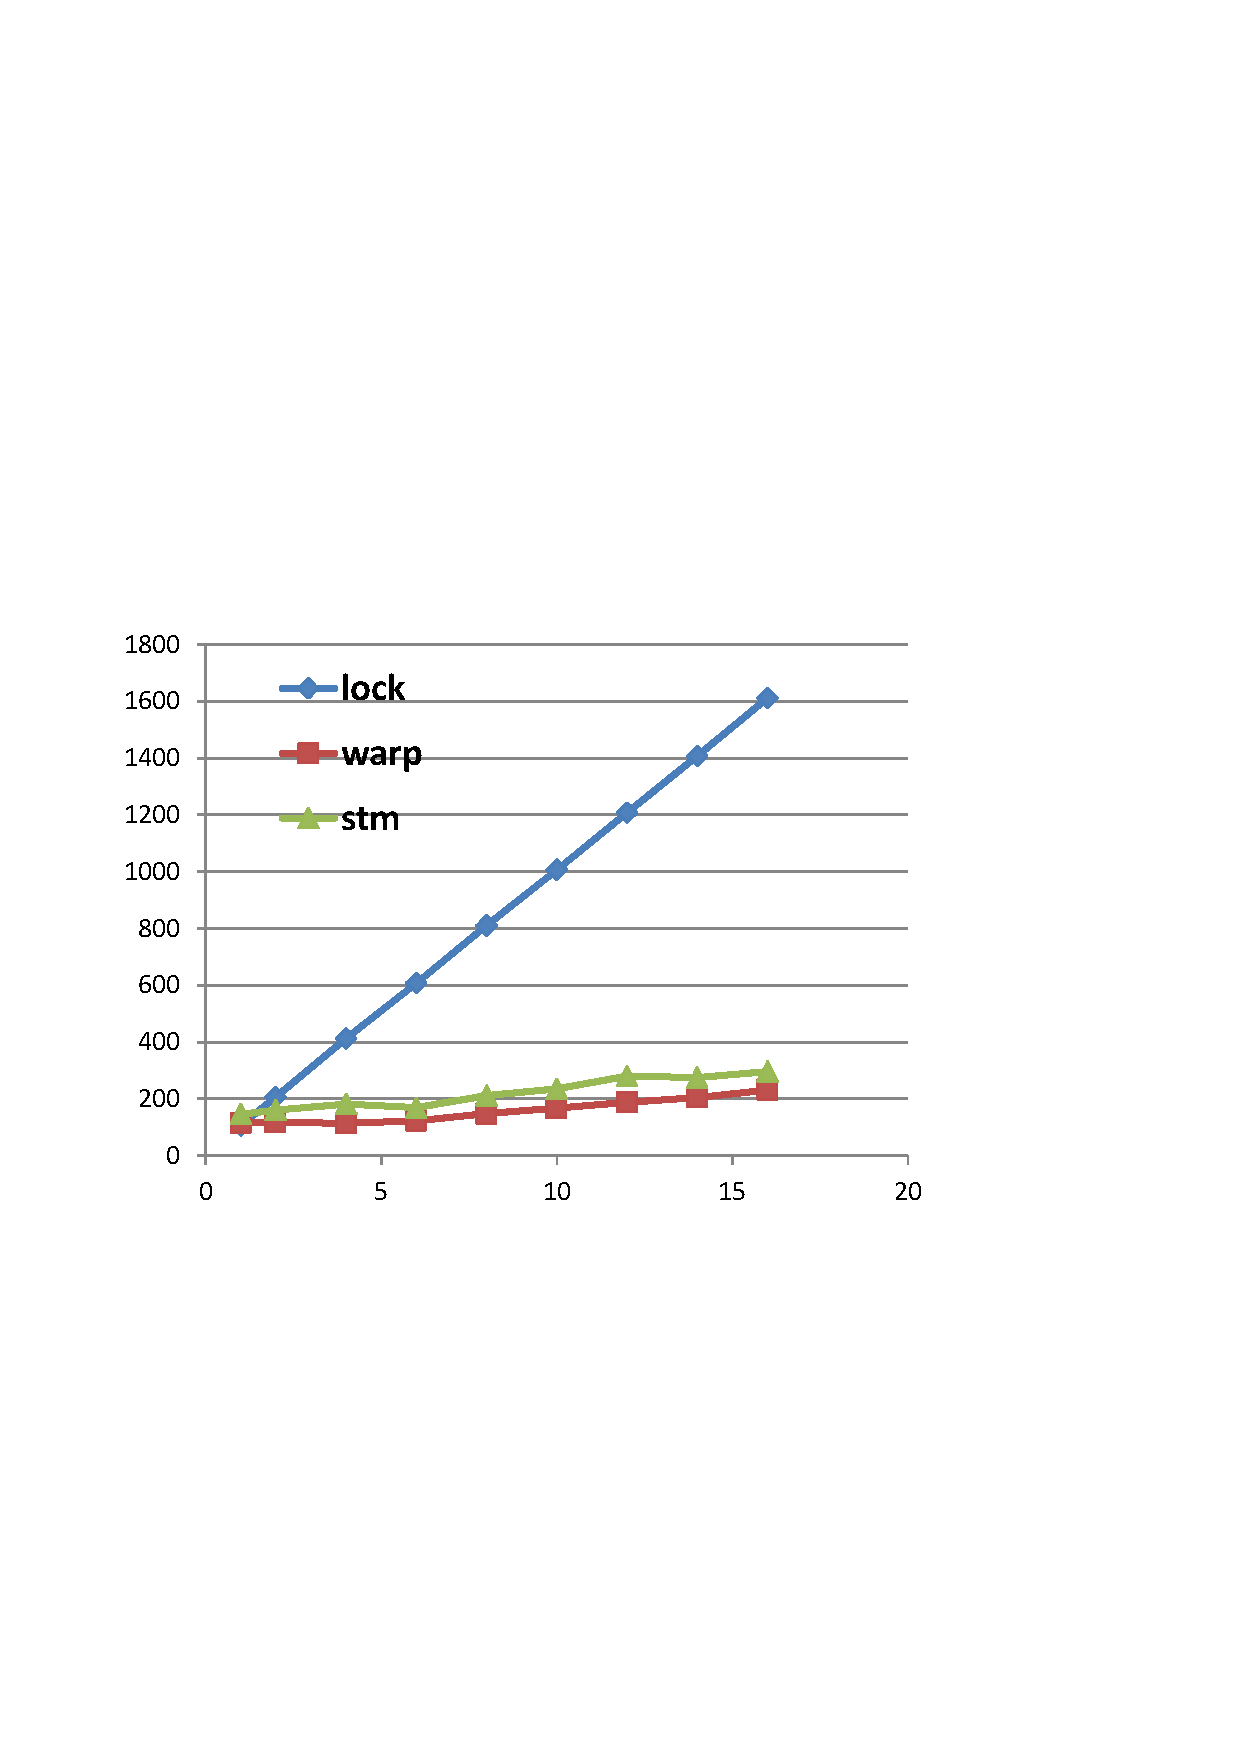
\includegraphics[width=0.33\textwidth]{../../eval/case5-varyThreads.pdf}}
%\caption{Performance Measurement}
%\label{fig:perf}
%\vspace{-1em}
%\end{figure*}







